% Version 0; preprint format; Written by SH
% Version 1; emulateapj format; Edited by SH and AL
% Version 2; emulateapj format; Edited by SH and AL
% Version 3; emulateapj format; Edited AL
% Version 4; emulateapj format; Edited SH
% Version 5; MNRAS format; Edited SH

\documentclass[a4paper,fleqn,usenatbib]{mnras}

% Packages
\usepackage{deluxetable}
\usepackage{newtxtext,newtxmath}
\usepackage[T1]{fontenc}
\usepackage{ae,aecompl}
\usepackage{amssymb, amsmath}
\usepackage{graphicx}
\usepackage{natbib}
\usepackage{url}
\usepackage{hyperref}
\usepackage{float}
\usepackage[usenames, dvipsnames]{color}

% Package Settings
\hypersetup{colorlinks=true,
            citecolor=cyan,
            linkcolor=cyan,
            filecolor=magenta,      
            urlcolor=cyan}
\urlstyle{same}

% Figure extention
\DeclareGraphicsExtensions{.pdf,.png,.jpg}

%%%%%%%%%%%%: User Defined Commands %%%%%%%%%%%%

% Song Huang's definition 
\def\arcsec{{\prime\prime}}
\def\arcmin{{\prime}}
\def\degree{{\circ}}
\def\h{\hskip -3 mm}
\def\aa{{A\&A}}
\def\aas{{ A\&AS}}
\def\aj{{AJ}}
\def\al{$\alpha$}
\def\bet{$\beta$}
\def\amin{$^\prime$}
\def\annrev{{ARA\&A}}
\def\apj{{ApJ}}
\def\apjs{{ApJS}}
\def\asec{$^{\prime\prime}$}
\def\deg{$^{\circ}$}
\def\ddeg{{\rlap.}$^{\circ}$}
\def\dsec{{\rlap.}$^{\prime\prime}$}
\def\cc{cm$^{-3}$}
\def\flamb{erg s$^{-1}$ cm$^{-2}$ \AA$^{-1}$}
\def\flux{erg s$^{-1}$ cm$^{-2}$}
\def\fnu{erg s$^{-1}$ cm$^{-2}$ Hz$^{-1}$}
\def\hst{{\textit{HST}}}
\def\kms{km s$^{-1}$}
\def\lamb{$\lambda$}
\def\lax{{$\mathrel{\hbox{\rlap{\hbox{\lower4pt\hbox{$\sim$}}}\hbox{$<$}}}$}}
\def\gax{{$\mathrel{\hbox{\rlap{\hbox{\lower4pt\hbox{$\sim$}}}\hbox{$>$}}}$}}
\def\simlt{\lower.5ex\hbox{$\; \buildrel < \over \sim \;$}}
\def\simgt{\lower.5ex\hbox{$\; \buildrel > \over \sim \;$}}
\def\micron{{$\mu$m}}
\def\mnras{{MNRAS}}
\def\nat{{Nature}}
\def\pasp{{PASP}}
\def\perang{\AA$^{-1}$}
\def\peryr{yr$^{-1}$}
\def\reference{\noindent\pp}
\def\refindent{\par\noindent\parskip=2pt\hangindent=3pc\hangafter=1 }
\def\sb{mag~arcsec$^{-2}$}
\def\lsun{$L_\odot$} 
\def\msun{$M_\odot$}
\def\sigs{$\sigma_*$}
\newcommand{\lt}{<}
\newcommand{\gt}{>}

\def\etal{{\ et al.~}}
\def\galfit{{\tt GALFIT}}
\def\ser{{S\'{e}rsic\ }}
\def\redm{\texttt{redMaPPer}}
\def\cmodel{\texttt{cModel}}
% Samples
\def\rbcg{\texttt{cenHighMh}}
\def\nbcg{\texttt{cenLowMh}}
\def\redbcg{{$\lambda \ge 30$}}
\def\nonbcg{{$\lambda < 20$}}
% Mass related 
\def\mstar{{$M_{\star}$}}
\def\mhalo{{$M_{\mathrm{halo}}$}}
\def\logms{{$\log (M_{\star}/M_{\odot})$}}
\def\logmh{{$\log (M_{\mathrm{halo}}/M_{\odot})$}}

\def\minn{{$M_{\star,10\mathrm{kpc}}$}}
\def\meff{{$M_{\star,15\mathrm{kpc}}$}} 
\def\mtot{{$M_{\star,100\mathrm{kpc}}$}}
\def\mout{{$M_{\star,150\mathrm{kpc}}$}}
\def\mmax{{$M_{\star,\mathrm{Max}}$}}
\def\mgama{{$M_{\star,\mathrm{GAMA}}$}}
\def\mcmodel{{$M_{\star,\mathrm{cModel}}$}}

\def\logminn{{$\log (M_{\star,10\mathrm{kpc}}/M_{\odot})$}}
\def\logmtot{{$\log (M_{\star,100\mathrm{kpc}}/M_{\odot})$}}
\def\logmout{{$\log (M_{\star,150\mathrm{kpc}}/M_{\odot})$}}
\def\logmmax{{$\log (M_{\star,\mathrm{Max}}/M_{\odot})$}}
\def\logmgama{{$\log (M_{\star,\mathrm{GAMA}}/M_{\odot})$}}
\def\logmcmodel{{$\log (M_{\star,\mathrm{cModel}}/M_{\odot})$}}

\def\m2l{{$M_{\star}/L_{\star}$}}
\def\mden{{$\mu_{\star}$}}

% Commenting:
\newcommand{\xxx}[1]{\textcolor{red}{\textbf{XXX}}}
\newcommand{\todo}[1]{\textcolor{red}{\textbf{TODO:~#1}}}
\newcommand{\plan}[1]{\textcolor{cyan}{#1}}
\newcommand{\addref}{{\textcolor{red}{REF}}}
\newcommand{\note}[2]{\textcolor{blue}{\textbf{[Comment (#1): #2]}}}
\newcommand{\song}[1]{\textcolor{magenta}{\textbf{[Song: #1]}}}
\newcommand{\alexie}[1]{\textcolor{blue}{\textbf{[Alexie: #1]}}}
\newcommand{\kevin}[1]{\textcolor{green}{\textbf{[Kevin: #1]}}}
\newcommand{\update}[1]{\textcolor{Bittersweet}{#1}}
%\newcommand{\update}[1]{#1}


%%%%%%%%%%%%: Title and Affiliations %%%%%%%%%%%%

\title[Structure and Halo of Massive Galaxies]{A Detection of the Environmental 
       Dependence of the Stellar Halos of Massive Central Galaxies}

\author[S. Huang et al.]{
        Song Huang,$^{1,2}$\thanks{E-mail: song.huang@ipmu.jp (SH)}
        HSC collaboration$^{3}$   
        \\ \\
        % List of institutions
        $^{1}$Kavli-IPMU, The University of Tokyo Institutes for Advanced Study, 
              the University of Tokyo (Kavli IPMU, WPI), Kashiwa 277--8583, Japan\\
        $^{2}$Department of Astronomy and Astrophysics, University of California 
              Santa Cruz, 1156 High St., Santa Cruz, CA 95064, U.S.A\\
        $^{3}$Another Department, Different Institution, Street Address, City Postal 
              Code, Country
        }

\date{Accepted XXX. Received YYY; in original form ZZZ}        
\pubyear{2017}                                  
  
%        \author{Song Huang\altaffilmark{1} 
%        Alexie Leauthaud\altaffilmark{1}, 
%        Kevin Bundy\altaffilmark{1},
%        Michael Strauss\altaffilmark{2},
%        Yen-Ting Lin\altaffilmark{3},
%        Rachel Mandelbaum\altaffilmark{4}
%        }
%\altaffiltext{2}{Princeton University Observatory, 
%    Peyton Hall, Princeton, NJ 08544, USA}
%\altaffiltext{3}{Institute of Astronomy and Astrophysics, Academia Sinica, 
%    P.O.~Box 23--141, Taipei 10617, Taiwan}
%\altaffiltext{4}{Carnegie-Mellon University \todo{correct affiliation here}}

%%%%%%%%%%%%: Header and Version %%%%%%%%%%%%

\begin{document}

\label{firstpage}
\pagerange{\pageref{firstpage}--\pageref{lastpage}}

\maketitle

%%%%%%%%%%%%: Abstract and Keywords %%%%%%%%%%%%

\begin{abstract}
    
    The promising hierarchical assembly scenario of massive galaxies suggest the 
    structure of these galaxies should depend on their environments or halo mass.
    Yet, at low redshift, observations find no clear evidence for that. 
    Here, using the deep images from the Subaru Hyper Suprime-Cam (HSC) survey,
    we map the stellar mass distributions of massive galaxies at $0.3 < z < 0.5$ 
    out to the very outskirt, and detect subtle, but robust structural differences 
    that depend on halo mass for central galaxies at high mass end. 
    With the help of the \redm{} catalog, we separate these massive galaxies 
    into centrals of halos that are more and less massive than 
    $M_{\mathrm{Halo}}\sim 10^{14} M_{\odot}$.
    For centrals with similar stellar mass within 100 kpc, the ones from 
    more massive halos on average have slightly more flattened inner profile 
    within $\sim 10$-$20$ kpc, and more prominent outer envelope.
    Meanwhile, when matched at the same stellar mass within inner 10 kpc--a 
    proxy of the mass of the in-situ component, the massive centrals of more  
    massive halos show much more significant outer stellar envelopes.    
    We also see that these two samples of massive galaxies follow slightly 
    different mass-size relation and the relationship between the stellar mass 
    within 100 and 10 kpc.
    Such differences in structure are broadly consistent with the expectation that
    central galaxy from more massive halo should have more complex merging history.
    These results highlight the importance of deep photometry in the study of 
    the assembly history of massive galaxies.  

\end{abstract}

\begin{keywords}
    galaxies: elliptical and lenticular, cD --
    galaxies: formation --
    galaxies: photometry -- 
    galaxies: structure -- 
    galaxies: surveys
\end{keywords}


%%%%%%%%%%%%: Main Text %%%%%%%%%%%%

%% ------------------------------------------------------------------------------------ %% 
    \begin{figure*}
        \centering 
        \includegraphics[width=\textwidth]{fig/redbcg_sdss_compare}
        \caption{
            A comparison between the depth and imaging quality of SDSS and the HSC wide 
            layer for a sample of nearby massive elliptical galaxies at $0.2 < z < 0.5$.  
            These images are generated using $gri$ band images with an arcsinh stretch 
            \citep{Lupton2004}. 
            The HSC \texttt{WIDE} layer is $3.0$-$4.0$ magnitudes deeper than SDSS.
            This added depth is critical in order map the outskirts of ETGs out to 
            large radii.
            }
        \label{fig:sdss_compare}
    \end{figure*}
%% ------------------------------------------------------------------------------------ %% 

%% ------------------------------------------------------------------------------------ %% 
  \begin{figure*}
      \centering 
      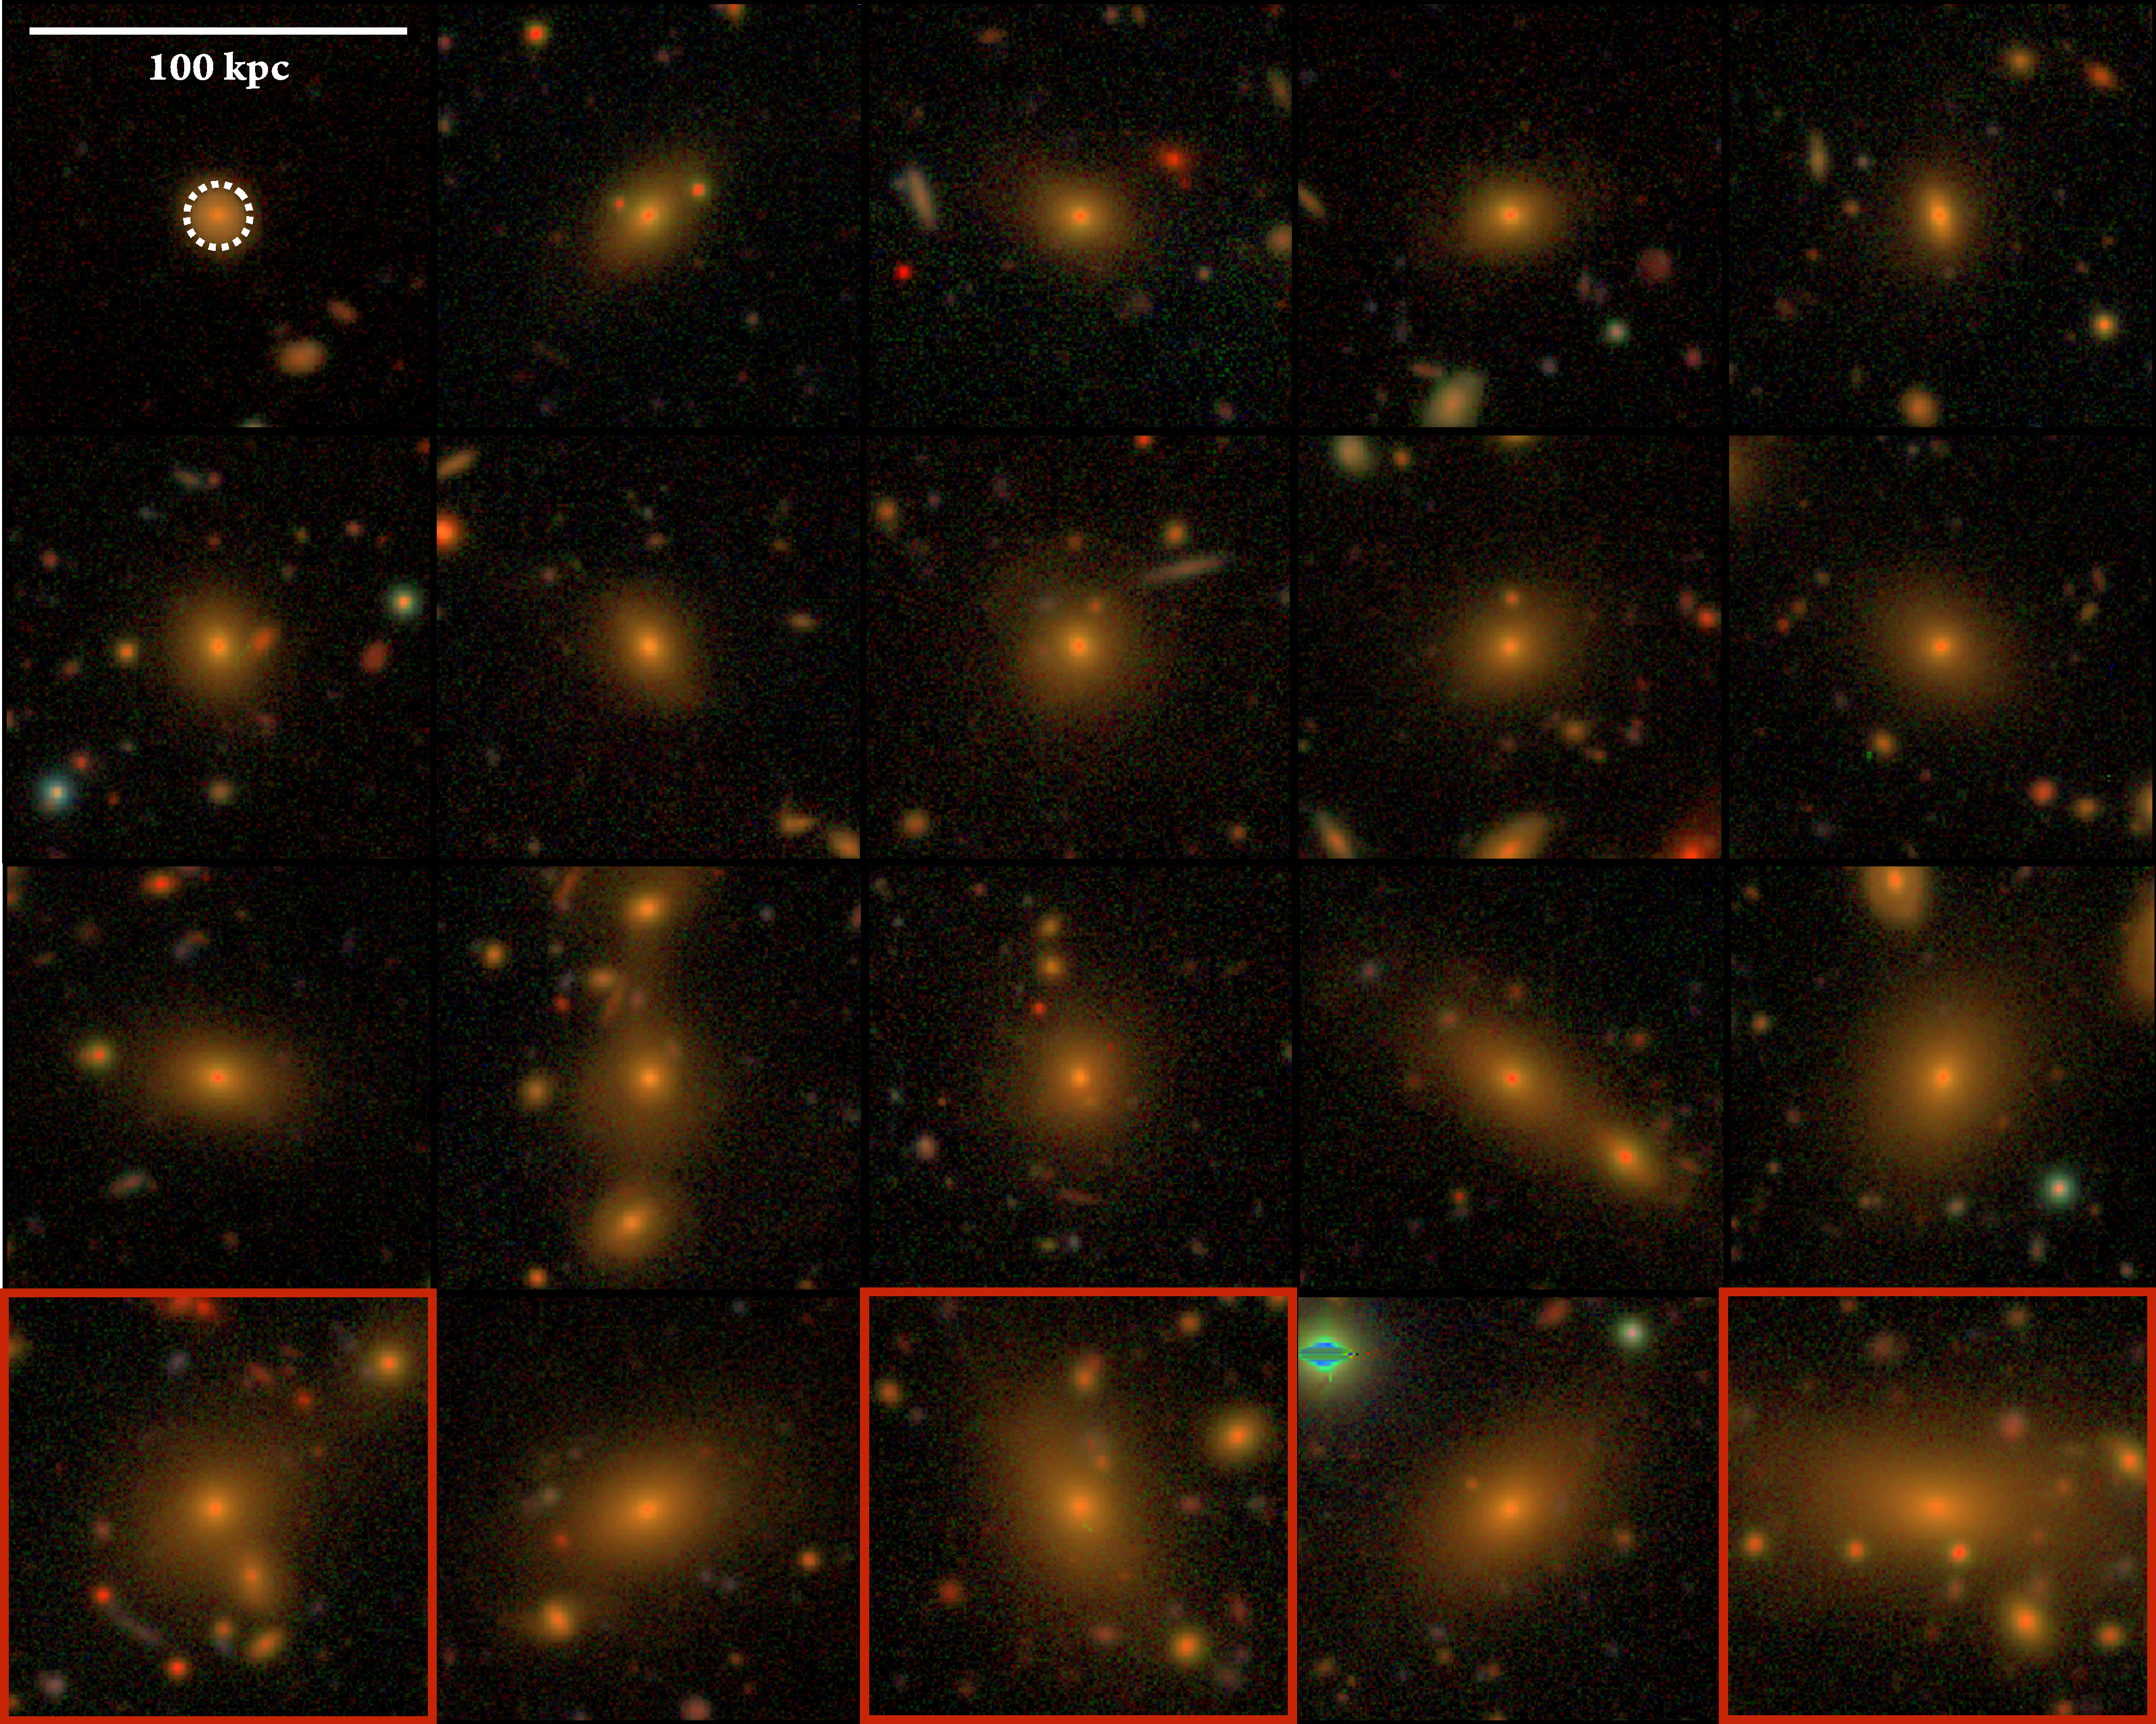
\includegraphics[width=\textwidth]{fig/redbcg_m100_m10_compare}
      \caption{
          Three-color images for a subsample of massive galaxies at $z\sim 0.4$. 
          All of these galaxies have the same mass within a 10 kpc aperture 
          ($11.2<\log (M_{\star,10\ \mathrm{kpc}}/M_{\odot})<11.3$). 
          The dash-line circle at the top-left figure indicates 10 kpc.
          Galaxies are rank-ordered from top to bottom and from left to right by 
          their \mstar{} within a 100 kpc aperture which varies from $10^{11.2} M_{\odot}$ 
          to $10^{11.7} M_{\odot}$. 
          At fixed "inner" mass ($M_{\star,10}$), massive galaxies display significant
          diversity in their outer profiles. 
          Red boxes indicate galaxies in halos more massive than 
          $\sim 10^{14.0} M_{\odot}$. 
          }
      \label{fig:m100_m10_color}
  \end{figure*}
%% ------------------------------------------------------------------------------------ %% 

%% ------------------------------------------------------------------------------------ %% 
\section{Introduction}
    \label{sec:intro}
    

    Massive galaxies are unique laboratories for studying both cosmology and galaxy 
    formation. 
    Simulations of structure formation within the context of the $\Lambda$-CDM 
    cosmological model make predictions for the hierarchical growth of dark matter halos 
    and galaxies (e.g. \citealt{Baugh1996, DeLucia2006}), but there are many open 
    questions regarding the star-formation history, mass assembly process, and 
    structural evolution of massive galaxies. 
    Massive galaxies are thought to grow according to a ``two-phase'' formation scenario 
    (e.g. \citealt{Oser2010, Oser2012}). 
    In this scenario, the progenitors of $z\sim 0$ massive early-type galaxies (ETGs) 
    undergo a rapid growth phase at $z\sim 2$ triggered either by disk instabilities 
    or gas rich mergers (e.g\citealt{Hopkins2008, Dekel2009}). 
    Observationally, the progenitors of ETGs are thought to correspond to the so-called 
    ``red nuggets'' (e.g. \citealt{Damjanov2009}) which have smaller effective radii 
    ($R_{\mathrm{e}}$; \citealt{Trujillo2006, vanDokkum2008, Cimatti2008}), 
    slightly higher central velocity dispersion and stellar mass density 
    (\mden{}; e.g. \citealt{vandeSande2011, Belli2014}), more disk-like morphologies 
    (e.g. \citealt{vanderWel2011}) than their local descendants 
    (e.g. \citealt{Bezanson2009, vanDokkum2010}).
    
    Following an initial epoch of early formation, feedback from stars and/or AGN 
    (e.g. \citealt{Sijacki2007, Fabian2012}) efficiently quench star formation in 
    massive galaxies and a large fraction of these massive progenitors become quiescent 
    at $z>1$ (e.g. \citealt{Bezanson2009, Kriek2016}). 
    The second phase in the ``two-phase'' formation scenario is driven by 
    non-dissipative processes such as dry mergers with other galaxies 
    (e.g. \citealt{Naab2006, Khochfar2006}). 
    According to the ``two-phase'' scenario, minor mergers drive the growth of massive 
    galaxies at late times and can help explain the significant increase
    of $R_{\mathrm{e}}$ (e.g. \citealt{Newman2012, vdWel2014}) as well as the build-up 
    of the outer stellar halos of ETGs (e.g.  \citealt{Szomoru2012, Patel2013}).         
   
    According to this two-phase formation scenario, the late time growth of massive ETGs 
    is intrinsically tied to the growth of their host dark matter halos 
    (e.g. \citealt{Leauthaud2012, Behroozi2013, Shankar2013}). 
    Massive ETGs that live at the center of more massive halos should experience 
    a different mass assembly history and should be subject to a larger merger rate 
    compared to ETGs that live in smaller dark matter halos. 
    A natural prediction of the two-phase formation scenario is therefore that the 
    structural properties of massive galaxies should depend on their ``environment''
    \footnote{There are different observational definitions of "environment". 
    In this paper, we use the term ``environment'' and halo mass interchangeably}.
    
    Previous work has shown that the half-light radii of massive ETGs is tightly 
    correlated with \mstar{} (e.g. \citealt{Shen2003, Guo2009}). 
    Models based on the ``two-phase'' formation scenario naturally predict that this 
    mass--size relation should exhibit an environmental dependence: the effective radii 
    of massive ETGs in more massive halos should be larger than those in less massive
    halos at fixed \mstar{} (e.g. \citealt{Shankar2013, Shankar2014}).
    
    However, while hints of an environmental dependence in the mass-size relation have 
    been spotted at high-$z$ (e.g. \citealt{Papovich2012, Lani2013, Delaye2014}; but 
    also see \citealt{Rettura2010}), there is no solid evidence for this effect at 
    low-$z$ (e.g. \citealt{Nair2010, HCompany13}; but also see \citealt{Yoon2017}). 
    The absence of an environmental dependence in the mass-size relation is an 
    outstanding challenge to the two-phase formation scenario of ETGs.
    
    From an observational perspective, we hypothesize that the lack of a detection of 
    this effect may be related a combination of the methodologies employed, as well as 
    the lack of deep high-quality imaging for large numbers of massive ETGs. 
    In particular, massive ETGs have very steep inner stellar density profiles, 
    extremely extended stellar envelopes, and radial-dependent isophotal shapes which 
    make accurate measurements of \mstar{} and $R_{\mathrm{e}}$ very challenging
    (e.g. \citealt{Bernardi2013, DSouza2014}), 
    especially in the presence of shallow imaging data such as the Sloan Digital Sky 
    Survey (SDSS; e.g. \citealt{SDSSDR7, SDSSDR12}). 
       
    In this paper, we take advantage of new high-resolution (median 
    FWHM$\sim 0.6^{\arcsec}$ in $i$-band) and deep ($i$-band surface brightness 
    limit $> 28.5$\sb) imaging from the Hyper-Suprime Cam (HSC) Subaru Strategic 
    Program (SSP; \citealt{HSCDR1; will be referred as the HSC survey} to revisit the 
    question of the environmental dependence in the mass-size relation. 
    The goal of this paper is to compare the \mden{} profiles and structural scaling 
    relations of massive central galaxies in both low and high mass dark matter halos. 
    Fig~\ref{fig:sdss_compare} displays a comparison of the imaging quality of massive 
    ETGs using SDSS versus using the new HSC data. 
    The deep imaging depth and excellent seeing conditions of HSC images make them 
    perfect for mapping the \mstar{} distributions of massive galaxies out to very 
    large radii. 
    With the help of the \redm{} cluster catalog (e.g.\ \citealt{Rykoff2014}; 
    \citealt{Rozo2015b}; please see Section~\ref{ssec:redmapper} for details), we 
    select a large sample ($\sim 15000$) of massive central 
    galaxies with $0.3 < z < 0.5$ using $\sim 100$ square degree of data from the 
    HSC wide layer.
    
    Motivated by the ``two-phase'' scenario, and also due to the difficulty in 
    providing appropriate model to describe the \mstar{} distribution of massive 
    galaxy from its center to the very outskirt, we focus on \mstar{} within two 
    different physical apertures in this work:
    
    \begin{itemize}
    
        \item The stellar mass within 10 kpc (hereafter noted \minn{}). 
            According to the two-phase scenario, the ``in-situ'' star-formation quickly 
            builds up the inner, dense core of massive ETGs.  
            Based on recent observations and simulations (e.g.~\citealt{vanDokkum2010}; 
            \citealt{RodriguezGomez2016}), the in-situ component of massive ETGs is 
            mostly contained within one effective radius ($R_{\mathrm{e}}$, or 5-10 kpc). 
            We use \minn{} as a proxy for the mass forged during the ``in-situ''
            phase. 
            Given the quality of the HSC data, we can reliably measure \minn{} over our 
            redshift range ($1.0^{\arcsec}$ in radius equals 4.4 and 6.1 kpc at redshift
            0.3 and 0.5).  
            
        \item The stellar mass within 100 kpc (hereafter noted \mtot{}). 
            For our galaxy sample, a 100 kpc aperture corresponds to 5-10 
            $\times R_{\mathrm{e}}$. 
            We show in section \ref{ssec:mtotal} that most of the mass for these ETGs 
            can be captured by a 100 kpc radius and that \mtot{} is a good proxy for the 
            ``total'' \mstar{}. 
            Although not perfect, we argue that our measurements of \mtot{} (which are 
            actually measuring the light directly out to 100 kpc) are a better tracer 
            of total \mstar{} than model-dependent results from shallower data 
            (such as SDSS) which rely on extrapolating the light profiles of galaxies 
            out to large radii.
            
       \end{itemize}
%% ------------------------------------------------------------------------------------ %% 
    
    Massive central galaxies in this work show an intriguing diversity on the plane 
    defined by these two metrics.  
    We preview this using Fig~\ref{fig:m100_m10_color}, which shows a subsample of 
    massive galaxies at $z\sim 0.4$ that share very similar value of \minn{}, but 
    exhibit a large diversity in their outer profiles. 
    Assuming that galaxies at fixed \minn{} share a similar in-situ formation history, 
    it is of great interest to investigate the relation between their present day halo 
    mass and the extend of their outer envelopes. 
    We note that although a circular aperture is shown on Fig~\ref{fig:m100_m10_color}, 
    for our mass measurements, we always use elliptical apertures that follow the 
    average isophotal shape. Finally, given our narrow mass and redshift range, we 
    can safely ignore significant mass growth and structural evolution in this work
    (no star formation, lower merger rate \etal~e.g.\ \citealt{Bellstedt2016},
    \citealt{Inagaki2015}; but also see \citealt{Bai2014}). 

    This paper is organized as follows. 
    Section \ref{sec:data} presents our data and our sample selection. 
    Section \ref{sec:ellipse} describes our procedure for extracting 1-D surface 
    brightness profiles. 
    Section \ref{sec:mstar} describes how we estimate stellar mass. 
    Our main results are presented in Section \ref{sec:result} and discussed in 
    Section \ref{sec:discussion}. 
    Section \ref{sec:summary} presents our summary and conclusions.

    Magnitudes use the AB system (\citealt{Oke1983}), and are corrected for Galactic 
    extinction using calibrations from \citet{Schlafly11}.
    In this work, we assume $H_0$ = 70~km~s$^{-1}$ Mpc$^{-1}$, ${\Omega}_{\rm m}=0.3$, 
    and ${\Omega}_{\rm \Lambda}=0.7$.
    Stellar mass is noted \mstar{} and has been derived using a Chabrier Initial Mass 
    Function (IMF; \citealt{Chabrier2003}).     
    $M_{\mathrm{halo}}$ denotes halo mass in general whereas $M_{\rm 200b}$ is 
    explicitly defined as $M_{\rm 200b}\equiv M(<r_{\rm 200b})=200\bar{\rho} 
    \frac{4}{3}\pi r_{\rm 200b}^3$ where $r_{\rm 200b}$
    is the radius at which the mean interior density is equal to 200 times
    the mean matter density ($\bar{\rho}$). 
    
%% ------------------------------------------------------------------------------------ %% 

%% ------------------------------------------------------------------------------------ %% 
    \begin{figure*}
        \centering 
        \includegraphics[width=\textwidth]{fig/redbcg_ellipse_example}
        \caption{
            Left: example of the 1-D surface brightness and ellipticity profile 
            for a massive galaxy at $z=0.23$ in the $i$-band using \texttt{Ellipse}. 
            In this work, we always show the radial profile using a $R^{1/4}$ scaling 
            on the x-axis. 
            By using this scale, the de Vaucouleurs profile will appear as a straight 
            line on this figure. 
            We also plot the relative brightness profile of the PSF model normalized 
            at the central surface brightness of the galaxy to highlight the region 
            affected by seeing. 
            The grey shaded region highlights the region most affect by seeing 
            ($r<3$ kpc).
            On the top panel, the dash line shows the ellipticity used for the final 
            isophote. 
            Right: the three color image of this galaxy with isophotes 
            extracted by \texttt{Ellipse}. 
            The thick dotted line highlights the isophote with 
            $\mu_{i}\sim 28.5$~\sb.
            }
        \label{fig:ellipse}
    \end{figure*}
%% ------------------------------------------------------------------------------------ %% 

%% ------------------------------------------------------------------------------------ %% 
\section{Data And Sample Selection}
    \label{sec:data}

\subsection{The Hyper Suprime-Cam Survey}
    \label{ssec:hsc}

    The Subaru Strategic Program (SSP, \citealt{MiyazakiInPrep}) makes use of the new 
    prime-focus camera, the Hyper Suprime-Cam (HSC;~\citealt{Miyazaki2012}), on the 
    8.2-m Subaru telescope at Mauna Kea. 
    The ambitious multi-layer HSC survey takes advantage of the large field of 
    view (FoV;~1.5 deg in diameter) of this camera and will cover $\sim 1400$ deg$^2$ 
    in 5 broad bands ($grizY$) to a limiting depth of $r \sim 26$ mag 
    in the \texttt{WIDE} layer. 
    This work is based on the internal data release \texttt{S15B}, which covers 
    $\sim 100$ deg$^2$ in all 5-band to full \texttt{WIDE} depth.  
    The regions covered by this release overlap with a number of spectroscopic surveys 
    (e.g.\ SDSS/BOSS: \citealt{Eisenstein2011}, \citealt{Alam2015}; 
    GAMA: \citealt{Driver2011}, \citealt{Liske2015}).

    The HSC \texttt{WIDE} survey is about $3.0$-$4.0$ magnitudes deeper in the $i$-band 
    than SDSS. 
    Combined with the excellent imaging resolution (the median $i$-band seeing is 0.6"), 
    and the wide area, the HSC survey represents a tremendous data set to perform a 
    large statistical study of the surface brightness profiles of ETGs out to large radii.     
    Fig~\ref{fig:sdss_compare} illustrates the quality of HSC imaging compared to SDSS 
    for three low redshift ETGs, and shows that HSC survey data are well suited for 
    mapping the stellar distribution of massive galaxies out to large radii.

	HSC $i$-band images typically have the best seeing compared to other bands because 
	of strict requirements driven by weak lensing science. 
    We will therefore use the $i$-band images to measure the stellar distributions of 
    massive galaxies.
    
%% ------------------------------------------------------------------------------------ %% 
\subsection{HSC Data Processing}
    \label{sec:pipeline}

    The full details of the HSC data processing can be found in \citet{BoschInPrep}
    and are briefly summarized here. 
    The HSC SSP data are processed with \texttt{hscPipe 4.0.1}, a derivative of the 
    Large Synoptic Survey Telescope (LSST) pipeline (e.g.\ \citealt{Juric2015}; 
    \citealt{Axelrod2010}), modified for HSC. 
    \texttt{hscPipe} first performs a number of tasks at the single exposure level 
    (bias subtraction, flat fielding, background modeling, object detection and 
    measurements). 
    Astrometric and photometric calibrations are performed at the single exposure level. 
    \texttt{hscPipe} then warps different exposures on to a common World Coordinate 
    System (WCS) and combines them into coadded images. 
    At this stage, \texttt{hscPipe} updates the images with a better astrometric and 
    photometric calibration using stars that are common among exposures. 
    
    The pixel scale of the combined images is $0.168^{\arcsec}$. 
    Photometric calibration is based on data from the Panoramic Survey Telescope 
    and Rapid Response System (Pan-STARRS) 1 imaging survey 
    (\citealt{Schlafly2012}, \citealt{Tonry2012}, \citealt{Magnier2013}). 
    To achieve consistent deblending and photometry across all bands, \texttt{hscPipe} 
    performs multi-band post-processing at the coadd level. 
    First, \texttt{hscPipe} performs object detection on coadd images in each band 
    independently and records the flux peak and the above-threshold region 
    (referred as a ``footprint'') for each source. 
    Next, ``footprints'' and peaks from different bands are merged together before     
    performing deblending and measurements. 
    Finally, \texttt{hscPipe} selects a reference band for each object based on the 
    $S/N$ in different bands (for most galaxies in this work, the reference band is 
    the $i$-band). 
    After fixing the centroids, shape, and other non-amplitude parameters of each 
    object in this reference catalog, \texttt{hscPipe} perform forced photometry 
    on the coadd image in each band. 
    This forced photometry approach is optimized to yield accurate galaxy colors. 
       
    For each galaxy, \texttt{hscPipe} measures a \cmodel{} magnitude using an approach 
    that is similar to SDSS (\citealt{BoschInPrep}). 
    However, as opposed to SDSS, the HSC \cmodel{} is based on forced photometry which 
    means that it can accurately measure both the \textit{fluxes and colors of galaxies}. 
    The HSC \cmodel{} algorithm fits the flux distribution of each object using a 
    combination of a de~Vaucouleur and an exponential component and accounts for the PSF. 
    The performance of this algorithm has been tested using synthetic objects 
    (\citealt{SynPipeInPrep}), and the results indicate that, generally speaking, 
    the HSC \cmodel{} photometry is accurate down to $i >25.0$ mag.  
    However, \cmodel{} currently systematically underestimates the total fluxes of 
    massive ETGs with extended stellar distributions. 
    This is caused by an intrinsic limitation of \cmodel{} as it is incapable of
    modeling profiles with extremely extended outskirts, a problem that is exacerbated 
    at the depth of the HSC survey. 
    In addition, at the depth of the HSC survey, accurate deblending in the vicinity of
    large ETGs where satellites and background galaxies often blend with the low surface 
    brightness stellar envelope is a challenging problem. 
    The deblending method implemented by the \texttt{hscPipe} currently tends to 
    ``over-deblend'' the outskirts of bright galaxies and leads to an 
    under-estimation of the the total flux of massive ETGs (this is discussed further in 
    \citealt{BoschInPrep}).  
    For these reasons, our results will be based on custom developed code to measure 
    the luminosities and stellar masses of massive galaxies. 
    We use the HSC \texttt{hscPipe} photometry for two purposes: 
    1) to perform a first broad sample selection, and 2) to estimate the average 
    color of massive galaxies.
    
%% ------------------------------------------------------------------------------------ %% 
\subsection{Initial Massive Galaxy Sample}
    \label{ssec:initial}
    
    We begin by using a broad luminosity cut to select an initial sample of massive 
    galaxies at $z < 0.5$ from the HSC photometric catalog. 
    Based on \citep{Leauthaud2016}, galaxies with \logms{}$\geq 11.5$ mostly have 
    $i_{\mathrm{SDSS, cModel}} \leq 21.0$ mag. 
    We therefore select our initial sample to be brighter than 
    $i_{\mathrm{HSC, cModel}} \leq 21.5$\footnote{We neglect small differences between 
    the response curves of SDSS-$i$ and HSC-$i$ filters.}
    and also limit our sample to regions that have reached the required depth of 
    the \texttt{WIDE} survey in the $i$-band.
    %% The SQL search is saved as "sample.sql" 
    %% The master catalog used here is "dr1_wide_galaxy_icmodel_21.5.fits"
    %%   The original catalogs contain 2275477 objects
    
    We further select extended objects with no deblending errors, with well defined 
    centroids, and with \texttt{cModel} magnitudes in all five bands. 
    After removing objects that have pixels affected by saturation, cosmic-rays, or 
    other optical artifacts\footnote{each criterion removes less than 8\% of the 
    entire sample.}.This sample corresponds to 1760845 galaxies and will be referred 
    as \texttt{hscPho}. 
    %% Saved as "dr1_wide_galaxy_hscPho.fits"      
        
    Here we limit our study to the very high-mass end where the majority of galaxies 
    have either a spectroscopic redshift or a robust red-sequence photo-$z$ from the 
    \redm{} catalog (see Section \ref{ssec:redmapper}).  
    We match the \texttt{hscPho} sample with a spec-$z$ catalog compiled by the HSC 
    team\footnote{It is created by matching HSC objects with all publicly available 
    spectroscopic redshifts (e.g.\ SDSS/BOSS; GAMA). The spec-z quality flag from 
    different catalogs are homogenized into a single flag that indicates secure 
    redshifts.}.  
    To ensure reasonable \mstar{}-completeness at the high-\mstar{} end we focus on
    the redshift range $0.3 \leq z \leq 0.5$. 
    %% This is catalog: "dr1_specz_use.fits"   
   
    For objects without a spectroscopic redshift, we match them with the central 
    galaxies from the \redm{} catalog using a $2.0^{\arcsec}$ matching radius. 
    The matched objects with useful red-sequence photo-$z$ ($z_{\lambda}$) are also 
    included in the final sample of bright galaxies with reliable redshift between 
    $0.3 \leq z \leq 0.5$. The accuracy of the red-sequence photo-$z$ is sufficient 
    (median $|z_{\lambda} - z_{\mathrm{Spec}}| \sim 0.01$ for the ones with a 
    spec-$z$) for the goal of this work.
    The \redm{} catalog provides an additional 133 unique redshifts for massive 
    galaxies in our sample.
    %% Estimated from "dr1_redbcg_hsc_sdss_gama_1arcsec.fits"
        
    In the end, at $0.3 \leq z \leq 0.5$, we gather a sample of 25286 galaxies with 
    reliable redshift information (will be referred as \texttt{hscZ}).
    %% Saved as "dr1_wide_galaxy_icmodel_21.5.fits"
    Among them, the BOSS and SDSS "legacy" LRG samples provide the majority of 
    spec-$z$. 
    By comparing with the Stripe 82 Massive Galaxy Catalog
    (\texttt{S82-MGC}; \citealt{Bundy2015}), \citet{Leauthaud2016} have measured the
    \mstar{} completeness of the combined BOSS and SDSS samples. 
    They estimate that the BOSS spec-$z$ sample is about 80\% complete at 
    \logms{}$\geq 11.6$ at $0.3 < z < 0.5$. 
    The GAMA survey, which partially overlaps with the HSC footprints, supplements 
    our \texttt{hscZ} sample by 14\%. 
    Based on \citet{Taylor2011} (e.g.\ their Fig~~6), at $z\sim 0.3$, the GAMA 
    sample is 80\% complete down to $10^{10.8}$\msun; but only 80\% complete to 
    $10^{12.0}$\msun at $z\sim 0.5$. 
    We can therefore expect our sample to be roughly \mstar{}-complete above 
    \logms{}$\geq 11.5$-$11.6$. 
    This question will be addressed more carefully using the overlap region between 
    HSC and the \texttt{S82-MGC} in Section \ref{ssec:s82}.

%% ------------------------------------------------------------------------------------ %%  
\subsection{The \redm{}{} cluster catalog}
    \label{ssec:redmapper}
    
    Our study focuses on galaxies located at the center of their dark matter halos. 
    To limit our sample to central galaxies, we use \texttt{v5.10} of the \redm{}{} 
    cluster catalog\footnote{See: http://risa.stanford.edu/redmapper/} 
    (e.g.\ \citealt{Rykoff2014}; \citealt{Rozo2015b}). 
    These authors have developed a well-tested red-sequence cluster finder that has 
    been run on SDSS DR8 (\citealt{SDSSDR8}) photometric data. 
    For each cluster, the catalog provides a photometric redshift ($z_{\lambda}$), a 
    cluster richness ($\lambda$), and identifies the most likely central galaxy (the 
    galaxy with the highest $P_{\mathrm{Cen}}$ value). 
    The \redm{}{} catalog also provides a list of member galaxies for each cluster and 
    their associated membership probabilities. 
    Details about the performance of the \redm{}~cluster catalog can be found in 
    \citet{Rozo2014}, \citet{Rozo2015a}, and \citet{Rozo2015b}. 
    Several studies have published calibrations between the \redm{}~richness estimate, 
    $\lambda$, and halo mass (e.g.\ \citealt{Saro2015, Farahi2016, Simet2016, 
    Melchior2016}). 
    All these studies consistently find that \redm{} clusters with $\lambda > 20$ 
    have $\log (M_{\mathrm{halo}}/M_{\odot}) \geq 14.0$. 
    The \redm{} catalog therefore helps us group massive central galaxies into 
    samples with different average \mhalo{}. 
    We will use the central galaxies of \redm{} clusters 
    ($P_{\mathrm{CEN}} \geq 0.7$) to form a sample of massive central galaxies that 
    live in massive halos.
    
    Due to the depth and resolution of SDSS, the \redm{} catalog becomes slightly 
    incomplete at lower richness ($\lambda < 40$) at $z > 0.33$. 
    To ensure a clean separation in \mhalo{}, here we only focus on the central 
    galaxies of clusters with $\lambda > 30$. 
    According to \citet{Simet2016}, this $\lambda \geq 30$ sample should correspond to 
    $M_{\mathrm{halo}}>10^{14.2} M_{\odot}$. 
    We have checked that none of the results in this work depend on the choice of this 
    $\lambda$ limit. 
    For massive central galaxies that are not in these cluster-level halos, 
    we unfortunately can not estimate their \mhalo{} individually, but it is safe 
    to assume they will have $\log (M_{\mathrm{halo}}/M_{\odot}) < 14.0$.  
%% ------------------------------------------------------------------------------------ %% 

%% ------------------------------------------------------------------------------------ %% 
  \begin{figure*}
      \centering 
      \includegraphics[width=\textwidth]{fig/redbcg_smf_new}
      \caption{
          \textbf{Left:} Difference between \mcmodel{} and \mtot{} for central
      	  galaxies in halos less massive than $10^{14} M_{\odot}$ (grey dots) and 
      	  in halos more massive than $10^{14} M_{\odot}$ (red squares). 
          On average, \mcmodel{} underestimates the total stellar mass of massive 
          galaxies by 0.1 dex while in some cases, the difference can exceed 0.2 dex.
          Vertical histograms indicate the mass difference for galaxies with
          $11.6<$\logmtot{}$<11.9$. 
          \textbf{Right:}: Impact of using \mcmodel{} on the galaxy stellar mass
          function. 
          Dashed lines correspond to the SMF computed using \mcmodel{} as an estimate
          of the total luminosity whereas solid lines correspond to the SMF computed
          using the total luminosity from our 1-D profile. 
          The impact on the SMF can exceed 0.2 dex for massive central galaxies 
          living in halos larger than $\log (M_{\mathrm{halo}}/M_{\odot}) > 14.2$ 
          (red lines).
          }
      \label{fig:smf1}
  \end{figure*}
          
%% ------------------------------------------------------------------------------------ %%
 
%% ------------------------------------------------------------------------------------ %% 
\subsection{Massive Central Galaxies in Low and High Mass Halos}
    \label{ssec:mass_central}

    Based on recent constraints of $M_{\star}$-$M_{\mathrm{Halo}}$ relation 
    (e.g.\ \citealt{Leauthaud2012}, \citealt{Behroozi2013}, \citealt{Kravtsov2014}), 
    even though our sample selects very massive galaxies (\logms{}$\geq 11.5$), they 
    live in a fairly broad range of halos masses.
    With the help of the \redm{} catalog, we can broadly separate our sample into two
    groups with \logmh{}$<14.0$ and \logmh{}$>14.2$.
    
    % We match this sample with the central galaxies of \redm{}~catalogs using a 
    % $1.0^{\arcsec}$ radius, and it results in 704 galaxies.  
    %% Saved as "dr1_redbcg_hsc_sdss_gama_1arcsec.fits"
    
    We match the \texttt{hscZ} sample with the central galaxies of \redm{} clusters 
    with $\lambda \geq 30$ and $P_{\mathrm{0.7}} \geq 0.7$, and find 164 matched 
    galaxies at $0.3 \leq z \leq 0.5$.
    Our sample of \textbf{central galaxies in more massive halos} will be referred to 
    as the \rbcg{} sample. 
    The median $\lambda$ of the clusters associated with the \rbcg{} sample is 
    $\sim 41$, corresponding to halo mass of 
    $M_{\mathrm{halo}}\sim 2.2\times 10^{14}$ $h^{-1}$ $M_{\odot}$.
    Only 44 centrals from the \rbcg{} sample live in clusters with $\lambda \geq 50$
    ($M_{\mathrm{halo}} \sim 3.0\times 10^{14}$ $h^{-1} M_{\odot}$). 
    Our \rbcg{} sample therefore corresponds to galaxies in moderate mass halos.
    %% Saved as "dr1_redbcg_use_sed5b.fits"
    
    Out next goal is to construct a sample of central galaxies living in halos with 
    \logmh{}$<14.0$. 
    We first identify and remove all galaxies within a cylindrical region around all 
    \redm{} clusters. 
    We use a radius equal to $R_{\mathrm{200b}}$ and the thickness of the cylinder is 
    set to twice the uncertainty of the photometric redshift error. 
    We convert $\lambda$ to $M_{\mathrm{halo}}$ using the calibration of 
    \citet{Simet2016} and we use the mass-concentration relation from 
    \citet{Diemer2015} to compute $R_{\mathrm{200b}}$. At $0.3 < z < 0.5$, the 
    uncertainty of photo-$z$ is between 0.015 to 0.025, and is enough to exclude 
    cluster members.
    After removing galaxies associated with \redm{} clusters, the remaining galaxies 
    in our sample will be dominated by central galaxies living in halos with 
    \logmh{}$\leq 14.0$. 
    We will refer to this sample of \textbf{central galaxies in less massive halos}
    as the \nbcg{} sample.
   
    We note that at this stage, our \nbcg{} sample still contains galaxies with a 
    wide range of \mstar{} values. 
    Later on, once we have more accurate \mstar{} estimates, we will further limit this 
    sample to \logms{}$ > 11.5$. 
    At this very high mass end, and given that we have rejected satellites in \redm{} 
    clusters, any further satellite contamination can be safely neglected 
    (e.g. \citealt{Reid2014, Hoshino2015, Saito2016, vanUitert2016}).
    %% Saved as "dr1_nonbcg_use_sed5b.fits"
    % TODO: The actual number waits to be updated}
    
 
%% ------------------------------------------------------------------------------------ %% 

%% ------------------------------------------------------------------------------------ %% 
\subsection{Summary of Sample Construction}
    \label{ssec:sample}

    Using $\sim 100$ deg$^2$ of HSC data, we select a large sample of massive central 
    galaxies with reliable redshift information, and broadly separate them two 
    categories based on $M_{\mathrm{halo}}$.
    
    The following is a summary of our sample construction.
    
    \begin{itemize}
        \item \texttt{hscPho} sample: this parent sample consists of bright galaxies 
            with $i_{\mathrm{cModel}} \leq 21.0$, good quality imaging, and reliable 
            \texttt{cModel} photometry in all five HSC bands in the \texttt{S15B} 
            data release. 
        \item \texttt{hscZ} sample: we limit the \texttt{hscPho} sample to galaxies 
            with reliable redshift information. 
        \item \rbcg{} sample: we select a sample of 164 galaxies at 
            $0.3 \leq z \leq 0.5$ that are the central galaxies 
            in $\lambda > 30$ \redm{} clusters. 
            They represent the central galaxies in very massive halos 
            (\logmh{}$\geq 14.2$). 
        \item \nbcg{} sample: after excluding all cluster members from the 
            \texttt{hscZ} sample, we have 14661 bright galaxies at 
            $0.3 \leq z \leq 0.5$. 
            After applying an additional \mstar{} cut (see Section 
            \ref{ssec:isedfit}), this sample corresponds to central galaxies in 
            halos with \logmh{}$<14.0$.  
    \end{itemize}
    
    We now proceed to measure the luminosities and stellar mass profiles for 
    all galaxies in the \rbcg{} and \nbcg{} samples.
%% ------------------------------------------------------------------------------------ %% 

%% ------------------------------------------------------------------------------------ %% 
\section{Measurements of 1-D Surface Brightness Profiles}
    \label{sec:ellipse}
    
    Massive ETGs imaged at the depth of HSC are not well modeled by simple models such 
    as the de~Vaucouleurs model or a single \ser component model. 
    These models will fail to simultaneously capture the profile in both the inner and 
    the outer region and these models also cannot account for any radial variations in 
    ellipticity and position angle. 
    In principle, massive galaxies can still be described by more complex 
    models (e.g \citealt{Huang2013a, Huang2013b, Oh2017}), but they are still 
    sensitive to the choices of models (e.g. de~Vaucouleurs or \ser{} profile), 
    the number of components, initial guesses of parameters, and the internal 
    degeneracies among different parameters. 
    Background subtraction uncertainty can affect the 2-D model fitting dramatically, 
    especially for massive ETGs in our sample. 
    We therefore perform elliptical isophote fitting using the IRAF \texttt{Ellipse} 
    algorithm (Jedrzejewski 1987) to estimate the total luminosities of massive 
    galaxies and measure their one-dimensional profiles of stellar mass surface 
    density (\mden{}). 
    This 1-D method we adopt is less affected by the issues mentioned above. 
    Also, we will only study galaxies in the radial range where we are not sensitive 
    to either the PSF ($r<3-5$ kpc) or the background subtraction ($r>100$ kpc). 
        
    We prepare large $i$-band cut-outs for each galaxy that extend to 750 kpc in 
    radius, along with a bad pixel mask, and the PSF model. 
    These cut-outs include all of the light of the galaxy and are large enough to 
    also evaluate the background level. 
    We choose to use $i$-band images because they trace the stellar distributions of 
    massive galaxies at $0.3 \leq z \leq 0.5$ reasonably well 
    (the observed i-band corresponds to a rest-frame $g$ or $r$ band), but also 
    because they have better seeing and much lower background levels than the $z$ 
    and Y band images (although these in principle may be better tracers of \mden{}). 
    
    For each cut-out, to overcome the \texttt{hscPipe} ``over-deblending'' issue, we 
    use a customized procedure to detect and appropriately mask out neighbouring 
    objects. 
    Furthermore, \texttt{hscPipe} tends to over-subtract the background around 
    bright objects. 
    To correct for this over-subtraction, we first aggressively mask all objects 
    (including the central massive galaxy), and derive an empirical background 
    correction using \texttt{SExtractor}.
    Then, we run \texttt{Ellipse} on the background-corrected, masked cut-outs 
    following the methodology of \citep{Li2012}. 
    In short, we first fit each isophote using a free centroid and shape 
    (ellipticity and position angle). 
    We then fix the centroid (using the mean flux-weighted centroid) and estimate
    the mean ellipticity and position angles of all isophotes. 
    Finally, we extract a 1-D surface brightness profile along the major axis using 
    the mean ellipticity and position angle. 
    We correct these surface brightness profiles for Galactic extinction and 
    cosmological dimming, and integrate them to various radii to get the luminosity 
    within different physical (elliptical) apertures. 
    Fig~\ref{fig:ellipse} shows an example of the 1-D surface brightness and 
    ellipticity profile for a massive galaxy at $z\sim0.2$ and also highlights 
    a few isophotes.    

    We test our procedure using different mask sizes, different \texttt{Ellipse} 
    parameters, and with or without our background correction. 
    Based on these tests, we find that our 1-D surface brightness profiles are reliable 
    up to surfaces brightness levels of $>28.5$ \sb. 
    Beyond that, some of our profiles shows signs of truncation and/or large 
    fluctuations which are due to the uncertainty in the background subtraction. 
    We choose to limit our study to surface brightness levels up to $\sim 28.5$ \sb. 
    This is a conservative choice but already enables us to measure light profiles 
    out to $100$ kpc on a galaxy-by-galaxy basis (no stacking). 
    For more details about the technical details of how we use \texttt{Ellipse}, 
    please see Appendix~\ref{app:ellipse}.
    
    For physical (e.g.\ late-stage major merger) and unphysical (e.g.\ nearby foreground 
    galaxy or bright star) reasons, we can not extract reliable 1-D profiles for a small 
    fraction of massive galaxies because they are heavily masked out. 
    This is an intrinsic limitation of the 1-D method. 
    It affects $18/164$ of the \rbcg{} sample, and a smaller fraction of the 
    \nbcg{} sample. 
    It is worth noting that this excludes most major-merging massive galaxies. 
%% ------------------------------------------------------------------------------------ %% 
    
%% ------------------------------------------------------------------------------------ %% 
\section{Stellar Masses and Stellar Mass Density Profiles}
    \label{sec:mstar}
    
%% ------------------------------------------------------------------------------------ %% 
\subsection{Stellar Masses from SED Fitting}
    \label{ssec:isedfit}
   
    To convert luminosities into stellar mass, we assume that these massive galaxies 
    can be well described by an average \m2l{}. 
    This is a reasonable assumption considering that they are mostly dominated by 
    old stellar populations and are known to have shallow color gradients. 
    We will further justify this point by measuring their median color profiles in 
    Section \ref{ssec:ell_color}.

    We use the broadband Spectral Energy Distributions (SEDs) fitting 
    (see \citealt{Walcher2011} for a recent review) code 
    \texttt{iSEDFit}\footnote{http://www.sos.siena.edu/~jmoustakas/isedfit/} 
    (\citealt{Moustakas13}) to estimate the average \m2l{} and $k$-corrections using
    5-band HSC \cmodel{} fluxes.
    Although \cmodel{} tends to underestimate the total flux for bright, extended 
    objects, it can still yield accurate \emph{average} colors thanks to the 
    forced-photometry method that takes the PSF convolution into account
    (e.g. \citealt{SynPipeInPrep}). 

    \texttt{iSEDFit} takes a simplified Bayesian approach. 
    In short, it first generates a large grid of SEDs from synthetic stellar population 
    models by drawing randomly from the prior distributions of relevant parameters 
    (e.g. age, metallicity, dust extinction, and star formation history).
    Based on these models, it uses the observed photometry and redshift to compute the 
    statistical likelihood, and generates the posterior probability distribution 
    functions (PDF) for each parameter.  
    To get the best estimate of a given parameter, \texttt{iSEDFit} integrates the 
    full PDF over all the other nuisance parameters.
    Then, the median value and the 1-$\sigma$ uncertainty are derived based on the 
    marginalized PDF. 
    Please refer to \citet{Moustakas13} for technical details. 
    
    In this work, we derive average \m2l{} using the Flexible Stellar Population 
    Synthesis\footnote{http://scholar.harvard.edu/cconroy/sps-models}
    (FSPS; \texttt{v2.4}; \citealt{FSPS}, \citealt{Conroy2010}) model based on the MILES
    \footnote{http://www.iac.es/proyecto/miles/pages/stellar-libraries/miles-library.php}
    (\citealt{MILES1}, \citealt{MILES2}) stellar library and assuming a
    \citet{Chabrier2003} IMF between 0.1 to 100 \msun. 
    The star formation history (SFH) is assumed to follow a delayed-$\tau$ model with 
    stochastic star bursts (see Appendix~\ref{app:sed}). 
    This SFH is appropriate for massive galaxies at low redshifts 
    (e.g.\ \citealt{Kauffmann2003}). 
    For stellar metallicity, we assume a flat distribution between 0.004 to 0.03 
    (the highest value allowed by FSPS). 
    We adopt the \citet{Calzetti2000} extinction law with a order two Gamma 
    distribution of $A_{V}$ between 0 to 2 magnitude. 
    A majority of our galaxies are red and quiescent and our results are 
    not very sensitive to parameters related to the SFH or the internal dust extinction. 
    To achieve reasonable sampling across these parameters, we generate 250000 models. 
    
    We construct five band SEDs using the forced-photometry \cmodel{} magnitudes 
    corrected for Galactic extinction. 
    \cmodel{} only accounts for the statistical error on the flux measurement but does
    not account for systematic uncertainties in the model-fitting process. 
    It therefore underestimates the flux errors of bright galaxies. 
    Based on tests using synthetic objects, we find that the average accuracy of
    \cmodel{} for bright galaxy is roughly at the 1\% level in the $r$, $i$, $z$ bands, 
    and slightly worse in the $g$ and Y-band. 
    Therefore, we supply \texttt{iSEDFit} with simplified flux errors assuming 
    $S/N = 100$ for the $riz$ bands, and $S/N = 80$ for the $g$Y bands (on average, 
    images in $gY$ bands are shallower in depth and/or have higher background noise).  
    The typical uncertainty of \logms{} is around 0.08-0.10 dex at \logms$\sim 11.5$. 
    Please see Appendix~\ref{app:sed} for further details.
      
%% ------------------------------------------------------------------------------------ %%  

%% ------------------------------------------------------------------------------------ %% 
  \begin{figure*}
      \centering 
      \includegraphics[width=\textwidth]{fig/average_mass_profiles_fsps1_A}
      \caption{
          \textbf{Left}: Median \mden{} profiles in three total stellar mass bins. 
              Here we combine the two \rbcg{} and \nbcg{} samples together -- 
              the halo mass dependence of these profiles will be explored in subsequent 
              figures. 
              Thin grey lines show a random subset of individual profiles. 
              The shaded region highlights the region that could be affected by the PSF. 
              Two vertical lines indicate 10 kpc (thin, dotted line) and
              100 kpc (thick, dash line). ~~~ 
          \textbf{Right}: comparison between our \mden{} profiles, previous observations, 
              and simulations. 
              The solid cyan line shows the median profile of massive elliptical 
              galaxies at $z\sim 0$ from \citet[][]{Huang2013a}. 
              The red long-dashed line shows the median profile of massive galaxies at 
              $0.25 \leq z < 0.50$ observed by \textit{HST} from \citet[][]{Patel2013}. 
              The purple short-dashed line shows the median radial stellar distributions 
              in massive halos from simulation using the particle tagging method
              (\citealt{Cooper13}).}
      \label{fig:avg_prof}
  \end{figure*}
%% ------------------------------------------------------------------------------------ %% 

%% ------------------------------------------------------------------------------------ %% 
  \begin{figure*}
      \centering 
      \includegraphics[width=\textwidth]{fig/redbcg_prof_1}
      \caption{
          \mden{} profiles for \mtot{}-matched ($11.6<$\logmtot{}$<11.9$) and 
          \minn{}-matched ($11.2<$\logminn{}$<11.6$) samples. 
          Orange and red correspond to \rbcg{} and grey and black correspond to \nbcg{}. 
          The \mtot{}-matched samples are shown on the left and the \minn{}-matched 
          samples are shown on the right. 
          Thin lines show the \mden{} profile for individual galaxies. 
          Thick lines with shaded regions show the median profile for each sample with 
          uncertainties given by the shaded region. 
          The bottom panel highlights the differences between the two median profiles 
          (brown solid line and shaded region). 
          To test the significance of the differential profile, we perform statistical
          tests by comparing the median profiles of two random groups that are drawn 
          from the mixed sample, and have the same sizes with the matched \rbcg{} and
          \nbcg{} ones. 
          Repeating this process 5000 times, the median (black solid line), 1-$\sigma$ 
          (dark-grey shaded region) and 3-$\sigma$ (light-grey shaded region) ranges
          of these random differential profiles are shown on the bottom panel.}
      \label{fig:prof_1} 
  \end{figure*}
%% ------------------------------------------------------------------------------------ %% 

%% ------------------------------------------------------------------------------------ %%        
    \subsection{Stellar Mass Completeness}
    \label{ssec:complete}
    
    With the help of the \texttt{S82-MGC} (\citealt{Bundy2015}), we investigate the 
    \mstar{} completeness of our samples. 
    The \texttt{S82-MGC} sample matches the deeper SDSS photometric data in the 
    Stripe 82 region (\citealt{Annis2014}) with the near infrared data from the United 
    Kingdom Infrared Telescope Infrared Deep Sky Survey (UKIDSS; \citealt{Lawrence2007}). 
    The deeper photometry and better photo-$z$s make the \texttt{S82-MGC} sample complete 
    to \logms{}$\geq 11.2$ at $z<0.7$ which makes it sufficient to evaluate the 
    completeness of our HSC samples.
    
    There are 20453 \texttt{S82-MGC} galaxies that are also in the \texttt{hscPho} 
    sample at $0.3 \leq z_{\mathrm{s82}} \leq 0.5$. 
    We compute \mstar{} values for these galaxies using our fiducial 
    procedure\footnote{The \mstar{} using HSC photometry is in excellent with the 
    values derived from the \texttt{S82-MGC} which includes NIR data from UKIDSS; 
    \texttt{S82-MGC} also uses \texttt{iSEDFit} with similar assumptions.}. 
    The right side of Fig~\ref{fig:smf1} compares the SMFs of galaxies from 
    \texttt{S82-MGC} with the SMFs of galaxies from our two 
    samples\footnote{Errors on the SMFs are estimated via bootstrap resampling}. 
    Based on Fig~\ref{fig:smf1}, we conclude that our sample of massive galaxies is 
    reasonably complete down to \logms{}$\sim 11.6$ at $0.3 \leq z \leq 0.5$. 
    The \rbcg{} sample is less affected by completeness because we can utilize 
    photo-$z$s from \redm{}. 
    However, the completeness of the \nbcg{} sample is still limited by the 
    availability of spec-$z$s from BOSS.
    
    In this work, we will focus on the range $11.6 \le$ \logmtot{}$ \le 11.9$ 
    where our two samples are complete. 
    When comparing \nbcg{} and \rbcg{} we will also always make sure that the two 
    samples are well matched both in terms of \mstar{} as well as in terms of redshift. 
    Please see the next section and Appendix~\ref{app:match} for more details.
%% ------------------------------------------------------------------------------------ %%

%% ------------------------------------------------------------------------------------ %% 
\subsection{Stellar Mass Corrected for Total Luminosity}
    \label{ssec:mtotal}
    
    Using the best-fit stellar mass from \texttt{iSEDFit} (noted as as \mcmodel{}), 
    we estimate the average \m2l{} in the $i$-band, then use that \m2l{} to convert our 
    1-D luminosity density profiles into stellar mass density profiles. 
    We also convert our 10 and 100 kpc aperture luminosities into corresponding stellar 
    mass estimates (noted as \minn{} and \mtot{}).
    
    For the remainder of this paper, we will use \mtot{} as a proxy of ``total'' 
    stellar mass. 
    In Appendix~\ref{app:sedasic}, we briefly summarize the basic statistics of 
    the \rbcg{} and \nbcg{} samples using our estimates of \mtot{} and \minn{}.
    We confirm that both samples follow a similar and very tight ``red-sequence''. 
    Appendix~\ref{app:sed} describes the outputs from our SED fitting process 
    (average stellar age, metallicity, and internal dust extinction). 
    We do not utilize these quantities in this paper, but we have checked that they all 
    behave reasonably for both samples. 
    As expected, the integration of the 1-D profile out to very large radius recovers 
    more luminosity (stellar mass) compared to the \cmodel{}-based estimates. 
    This will be shown in Section \ref{ssec:s82}.
    
    Our methodology ignores any radial variations in \m2l{}. 
    It is well known that massive ETGs have negative optical color gradients indicating 
    gradients in \m2l{} \alexie{xxx} (e.g.\ \citealt{LaBarbera2012}; 
    \citealt{DSouza2015}). 
    These color gradients are shallow and smooth out to a few times of the effective 
    radius and color gradients at the outskirts are not yet well quantified. 
    More importantly, for the comparison between the \rbcg{} and \nbcg{} samples, 
    our results will be robust as long as there is \emph{no significant difference in the 
    average color gradient between the two samples}. 
    We have confirmed that this is indeed the case and this will be discussed in Section 
    \ref{ssec:ell_color}. 
    
    Our method for deriving total stellar masses is similar to the 
    method adopted by the GAMA survey (\citealt{Taylor2011, Kelvin2012}). 
    We have compared our \mstar{} values with those from GAMA and the results are given 
    in Appendix~\ref{app:gama}. 
    We find a systematic differences between the two \mstar{} estimates.
    It is likely that the GAMA models fail to capture the flux associated with the 
    outskirts of galaxies due to the limited depth of SDSS.     
%% ------------------------------------------------------------------------------------ %% 
 
%% ------------------------------------------------------------------------------------ %% 
\section{Results}
    \label{sec:result}

%% ------------------------------------------------------------------------------------ %%     
    \subsection{Impact of Missing Light on the Galaxy Stellar Mass Function}
    \label{ssec:s82}
    
    Different methods for estimating the ``total'' \mstar{} can have a large impact on 
    the high mass end of the galaxy stellar mass function (e.g. \citealt{Bernardi2013, 
    DSouza2014, DSouza2015, Bernardi2016a}). 
    Fig~\ref{fig:smf1} shows the SMF computed using both \mtot{} and \mcmodel{}. 
    As one can be seen from this figure, our careful 1-D approach recovers more flux 
    in massive galaxies than \texttt{cModel}. 
    More importantly, the average difference steadily increases with \mtot{} and also 
    has a dependence on \mhalo{}. 
    At \logms{} $>11.5$, the difference can be larger than 0.2 dex. 
    This difference relates to the intrinsic limitation of the \texttt{cModel} method 
    and also reflects the fact that more massive ETGs tend to have more extended 
    stellar mass distributions (e.g. \citealt{Graham2003}). 
    Generally speaking, the use of \mtot{} instead of the \mcmodel{} shifts the SMF 
    towards the higher-mass end and slightly modifies the high-mass slope. 
    The impact of missing flux is most prominent for the \rbcg{} sample.
    For studies about the SMF or other aspects of galaxy evolution based on 
    \cmodel{}-like photometry or shallower images, these effects can not be neglected.
%% ------------------------------------------------------------------------------------ %%  

%% ------------------------------------------------------------------------------------ %%
\subsection{Surface Mass Density Profiles}
    \label{ssec:sbp_compare}

%% ------------------------------------------------------------------------------------ %%
\subsubsection{General Trends and Comparison with Previous Work}
    \label{sssec:sbp_inter}
          
    Compared to the much discussed "mass-size" relation, the \mden{} profiles that we 
    have derived capture the full information about the structural properties of 
    massive galaxies. 
    We argue that by studying the shapes of these galaxy profiles directly, we can 
    by-pass outstanding questions about how to accurately define and measure the 
    "sizes" and "masses" of these massive galaxies. 
    Fig~\ref{fig:avg_prof} shows the median \mden{} profiles\footnote{The median 
    profiles along with their uncertainties are derived using bootstrap resampling 
    method} of massive galaxies at $0.3 < z < 0.5$ in three \mtot{} bins\footnote{Here 
    we ignore a small population of massive satellites \alexie{xxxx} in \redm{} clusters 
    we excluded from our sample. 
    The sample is clearly not complete in the lowest \mtot{} bin, but its median \mden{}
    profile is still useful to show the overall trend and to compare with previous 
    observations}. 
    As shown in the left panel of Fig~\ref{fig:avg_prof}, we can comfortably trace
    the \mden{} profiles of these massive galaxies out to 100 kpc 
    \textbf{individually}. 
    These median \mden{} profiles have moderate differences in the inner region, 
    but show significant differences in the outskirts with more massive galaxies 
    showing more prominent stellar envelopes. 
    Most of these massive galaxies ($\ge 10^{11.4} M_{\odot}$) are slowly-rotating 
    (e.g.\ \citealt{Cappellari13b}) giant ellipticals with ``boxy'' inner isophotal 
    shapes (e.g.\ \citealt{Kormendy2009}), and slightly flattened inner \mden{} 
    profiles (e.g.\ \citealt{Lauer07}). 
    But in the outskirts, the structure of these galaxies clearly does \textbf{NOT} 
    response to the increase of stellar mass in a self-similar way.
    As mentioned earlier, some of the \mden{} profiles show signs of unphysical 
    truncation and fluctuation related to inaccurate sky subtraction.  
    We exclude the profiles outside 100 kpc, even though the median \mden{} 
    profiles for the two more massive bins behave reasonably out to $\sim 200$ kpc. 
    
    
    The right panel of Fig~\ref{fig:avg_prof} compares our median profiles with a few
    past works.
    So far, the surface brightness profiles of massive galaxies out to such large 
    radii was mostly derived via image stacking technique that suffers from several 
    systematic issues (e.g. \citealt{Tal2011, DSouza2015}; but also see:
    \citealt{Capaccioli2015}); and the \mden{} profiles are even more rarely 
    available.
    \citep{Huang2013a} derived \mden{} profiles for a small sample of very 
    nearby ellipticals (within 100 Mpc; median \logms{}$\sim 11.3$ based on shallower 
    images) from the Carnegie-Irvine Galaxy Survey (CGS, \citealt{CGS1}) that are 
    only affected by seeing within $r < 1$ kpc. 
    This median \mden{} profile qualitatively agrees with the one for the lowest 
    \mtot{} bin in the inner region, but shows a slightly more prominent outer 
    envelope at $r > 15$ kpc. 
    While the small size of the CGS sample ($\sim 30$) and differences in the
    measurements of \mstar{} could explain this difference, it may also correspond 
    to evidence for build-up in the outskirts of massive galaxies from $z\sim 0.4$ 
    to $z=0$. 
    CGS images are deeper than SDSS images in the $r$-band, but the median 
    profile from \citep{Huang2013a} still only reaches $\sim 50$ kpc for $z\sim 0$ 
    massive galaxies.
    Meanwhile, our deep HSC images can reliably deliver individual \mden{} profiles 
    for $z\sim 0.4$ galaxies out to at least 100 kpc.  
    
    \citet{Patel2013} extracted a median \mden{} profile of massive ETGs at 
    $0.25 < z < 0.50$ using stacked \textit{HST}/ACS images. 
    These galaxies are selected at a constant cumulative number density and are 
    thought to be the progenitors of $z=0$ massive ETGs (e.g. \citealt{Leja2013}).  
    The median \mstar{} of the \citet{Patel2013} sample is $\sim 10^{11.2} M_{\odot}$, 
    but the shallower imaging depth and the differences in SED fitting 
    assumptions\footnote{\citep{Patel2013} uses the BC03 SSP model, which show an 
    average -0.1 dex difference with the FSPS one based on our tests.}
    can make them comparable to our galaxies in the lowest \mtot{} bin, and the 
    comparison of \mden{} profiles does confirm that. 
    The superb resolution of the \textit{HST}/ACS image means that the profile in
    \citet{Patel2013} is unaffected by the seeing even down to 1 kpc. 
    The good agreement between our profile and the one derived from HST image 
    shows that our profiles are robust at $r > 3$ kpc and that we can accurately 
    measure \minn{}.
    
    Finally, we also compare with the predicted median \mden{} profile of central 
    galaxies in massive halos ($13.5 < \log M_{200,c} < 14.0$) from cosmological 
    simulation where the \mden{} profiles of galaxies are calculated using the 
    particle-tagging technique (\citealt{Cooper10}). 
    Despite the poorer resolution, the simulated \mden{} profile is already quite 
    similar to the median \mden{} profile for the $11.6 <$ \logmtot{} $< 11.8$ bin 
    within 40 kpc. 
    However, compared with our data, this simulation predicts stellar envelope that
    are too prominent at this halo mass. 
    This types of comparisons between our HSC data and predictions from simulations 
    will help to fine-tune simulations and to also investigate the main physical 
    mechanisms that drive the assembly of massive galaxies and the build up of 
    stellar envelopes.

    Table 1 provides tabulated values for the median profiles that are displayed 
    in Fig~\ref{fig:avg_prof}. 
    These profiles are also available  
    \href{https://github.com/dr-guangtou/hsc_redbcg/tree/master/profiles}{here}:
    {\url{https://github.com/dr_guangtou/hsc_redbcg/tree/master/profiles/}}.
    
%% ------------------------------------------------------------------------------------ %% 

%% ------------------------------------------------------------------------------------ %% 
\subsubsection{Environmental Dependence of the \mden{} Profiles}
    \label{sssec:sbp_mtot}    
    
    Finally, we will look into the environmental dependence of structures in massive 
    galaxies using the \mden{} profiles of the \rbcg{} and \nbcg{} samples that are 
    carefully matched in \mstar{} and redshift using KDTree algorithm. 
    We discuss the details and quality of the matching procedure in 
    Appendix~\ref{app:match} (see Fig~\ref{fig:match}. 
    The matched redshift distributions within $0.3 < z < 0.5$ ensures the \mden{} 
    profiles from both samples are impacted by seeing and background at similar level. 
    As for the \mstar{}, we choose to match using two physically meaning definitions.
    
    \begin{itemize}
        \item \mtot{} as the proxy of the ``total'' \mstar{} that include the stellar 
            envelope.  As mentioned earlier, we match the two samples within 
            $11.6 < $\logmtot{}$<11.9$ (median \logmtot{}$\sim 11.74$).
            For the 45 \rbcg{} galaxies, we have 229 unique \nbcg{} galaxies in the 
            matched sample.
            Within this \mtot{} range, 100 kpc equals to 5-8 times of the effective 
            radius, so should enclose most their \mstar{}. 
            In practice, this choice also reflects the radius range that we can safely 
            measure \mden{} profile given the depth of the image and the accuracy of 
            background subtraction.
        
        \item \minn{} as the proxy of the \mstar{} of the ``in-situ'' component.
            This is motivated and supported by recent observations and simulations, 
            and we will discuss more about this assumption in 
            Section~\ref{sec:discussion}.
            We match the two samples within $11.2 < $\logminn{}$ < 11.6$ 
            (median \logminn{}$\sim 11.36$).
            For 56 galaxies in this \rbcg{} sample, we achieve excellent matches
            using 375 \nbcg{} galaxies.
    \end{itemize}
    
    We show the comparison of the \mtot{}-matched (\minn{}-matched) samples in the 
    left (right) panel of Fig~\ref{fig:prof_1}. 

    For the \mtot{}-matched comparison, it is easy to see that the \mden{}
    profiles of \rbcg{} and \nbcg{} galaxies \textbf{greatly overlap with each 
    other over the entire radius range}, which partially explains the difficulties in 
    confirming any environmental dependence of structure in earlier works.
    Although the central galaxies from more massive halos do not form a unique 
    population in term of their structures comparing with the ones in less massive
    halos at similar \mtot{}, we can still spot interesting differences in their 
    median profiles: the \rbcg{} galaxy on average has slightly more flattened inner 
    profile and more significant outer stellar envelope than the \nbcg{} one.
    We highlight these subtle differences in the bottom panel using the difference 
    between the two median profiles and its uncertainty. 
    Given the noticeable uncertainties of \mtot{} and $\lambda$, along with the 
    small size of the current \rbcg{} sample, we perform statistical test to confirm 
    the robustness of the result \footnote{We mix the $N_{\mathrm{r}}$ \rbcg{} 
    galaxies and the $N_{\mathrm{n}}$ \mtot{}-matched \nbcg{} ones together, then 
    randomly draw $N_{\mathrm{r}}$ galaxies with putting-back, compute the difference 
    between the median profile of this sample and the \nbcg{} sample. 
    After repeating this process 2000 times, we can evaluate the possibility that 
    the systematic differences in median \mden{} profiles can be reproduced by random 
    selection of massive galaxies.}
    In both inner and outer regions, we conclude the systematic differences in 
    median \mden{} profiles are significant and robust.
    Interestingly, the median profiles for \rbcg{} and \nbcg{} cross each other 
    at $\sim 15$-20 kpc, quite close to the expected $R_{\mathrm{e}}$ for ETGs 
    this massive. 
    In Appendix~\ref{app:robust}, we further prove the robustness of this 
    interesting result by showing that it is not affected by the range of redshift,
    range of richness, and the choice of proxy for ``total'' \mstar{} 
    (see Fig~\ref{fig:prof_3}). 
    We also explore the possible \mtot{}-dependence of this structural difference 
    despite the limitation of \mstar{}-completeness and small sample size
    (see Fig~\ref{fig:prof_2}) in Appendix~\ref{app:robust}.
    Although the systematic differences are very similar in different \mtot{} bins, 
    we do find some hints that suggest the environmental dependence becomes more 
    significant at the more massive end.  
    This evidence could have intriguing implication in the assembly history of 
    massive galaxies, and is worth more investigations with larger and more completed 
    sample later.  

    \textbf{All these tests confirm that we robustly detect subtle, but systematic 
    \mhalo{}-dependence (environmental dependence) of structure in massive, 
    central galaxies} that seems to be consistent with the expectation of more frequent 
    (minor) mergers in denser environment. 
    These minor, non-dissipative mergers do not alter the inner \mden{} profiles 
    a lot, but are efficient in depositing stellar mass onto the outer envelope
    (e.g. \citealt{Hilz2013}, \citealt{Oogi2013}).
    
%% ------------------------------------------------------------------------------------ %% 

%% ------------------------------------------------------------------------------------ %% 
    Meanwhile, the subtlety of this environmental dependence for \mtot{}-matched 
    samples seems to suggest that environment plays a secondary role in shaping 
    the structure of galaxies at fixed total stellar mass, and it encourages us to find
    another interesting angle.  
    For instance, for massive galaxies that formed similar amount of stars through 
    intensive star formation at high redshift, how the environments affect their mass 
    assembly history in the second phase? 
    We attempt to investigate this question through comparing the \mden{} profiles of 
    the \minn{}-matched \rbcg{} and \nbcg{} galaxies (right side of 
    Fig~\ref{fig:prof_1}).
    Assuming we are now comparing the average structures of massive galaxies that share 
    similar \mstar{} in the ``in-situ'' component, we start to see the environmental 
    dependence much more clearly without any statistical test.     
    The median \mden{} profiles of \rbcg{} and \nbcg{} galaxies are quite similar in 
    the inner 5-10 kpc, but the \rbcg{} galaxies clearly show much more prominent
    outer envelope.     
    
    It is also worth noting that \mden{} profiles of massive galaxies have quite uniform
    slope and small scatter inside 10 kpc.  
    In contrast, their outer profiles could have a large range of slopes and much 
    larger scatters than the inner region. 
    It seems to suggest that the inner and outer parts of massive galaxies are shaped 
    by distinctive physical processes, and are affected by their environment at 
    very different level. 
    Given the highly dissipative nature of the ``in-situ'' phase, the similarity of 
    inner profiles is consistent with the idea that processes like wet-merger and 
    star burst often create de~Vaucouleur-like ($n\sim 4$) \mden{} profile
    (e.g. \citealt{Hopkins2008}).
    At the same time, the outer envelope of massive galaxies are predicted to be 
    gradually assembled by non-dissipative mergers, which is a stochastic process and 
    is more affected by the environment.  
    Therefore, it is natural to see larger diversity in the outer profiles of 
    low-$z$ massive galaxies. 
    On average, massive galaxies in more massive halos show shallower outer \mden{} 
    profiles, which is in qualitative agreement with recent simulation
    (e.g. \citealt{Pillepich2014}).
    We illustrate this interesting diversity in Fig~\ref{fig:m100_m10_color}, where 
    we show the 3-color images of randomly selected massive central galaxies that 
    have similar \minn{} ($11.1 \leq \log (M_{\star,\ 10\mathrm{kpc}}/M_{\odot}) < 11.2$)
    but different \mtot{}.   
    From the top-left to the bottom-right, the \mtot{} of these galaxies increases
    from $10^{11.22} M_{\odot}$ to $10^{11.75} M_{\odot}$.
    
    As with the \mtot{}-matched sample, the results are very robust against 
    sample details, definition of ``inner'' \mstar{} and the \minn{} bins. 
    In Appendix~\ref{app:match}, we also show that:
    1) When we match using both \minn{} and \meff{}, we end up with \rbcg{} and \nbcg{} 
    samples with perfectly matched inner median \mden{} profiles, while the different 
    in the outskirt remains the same (see the left figure of Fig~\ref{fig:prof_4}).  
    2) Also, the results will not change even when only a more \mstar{}-complete sample
    (\logmtot{}$> 11.5$) is considered (see the right figure of Fig~\ref{fig:prof_4}). 
      
    The median profiles shown in Fig~\ref{fig:prof_1} are available in Table.1.
%% ------------------------------------------------------------------------------------ %% 

%% ------------------------------------------------------------------------------------ %% 
\subsection{Ellipticity and Color Profiles}
    \label{ssec:ell_color}
    
%% ------------------------------------------------------------------------------------ %% 
  \begin{figure*}
      \centering 
      \includegraphics[width=\textwidth]{fig/redbcg_discussion_2}
      \caption{
          Comparisons of the radial profiles of ellipticity and optical colors 
      	  for \mtot{}-matched (\textbf{left figure}) and \minn{}-matched 
      	  (\textbf{right figure}) of \rbcg{} (orange-red) and \nbcg{} (grey-black) samples. 
          The formats are very similar to the figure for \mden{} profile 
          (e.g. right figure of Fig~\ref{fig:prof_1}). 
          On each side, from top to bottom, we show the elliptical profile, and the 
          color profile using $g-r$ and $g-i$ color. 
          Since the individual profile of these properties has very large uncertain in the 
          outskirt, we block the region at large radii where we think the median profiles 
          are still unreliable using a dark, shaded box.
          We also compare these results with previous results based on SDSS images. 
          They are: 
          1) Ellipticity profile of the stacked image of a large sample of red galaxies at 
          $z\sim 0.4$ from \citet{Tal2011} with PSF correction 
          (solid blue line on top panel); 
          2) Ellipticity and $g-r$ color profiles from stacking analysis of nearby massive 
          galaxies with high concentration index ($C>2.6$) in \citet[][blue dash lines 
          on the top and middle panels]{DSouza2014}; 
          3) average $g-r$ and $g-i$ color profiles for a large sample of nearby 
          elliptical galaxies in \citet[][blue, solid lines on the middle and bottom 
          panels]{LaBarbera2010}.
          }
      \label{fig:ell_color}
  \end{figure*}
%% ------------------------------------------------------------------------------------ %% 
    
    Besides the 1-D \mden{} profiles, the radial profiles of isophotal shape and colors 
    are also useful diagnostic tools to study massive galaxies. 
    Here, we extract the radial profiles of ellipticity and $k$-corrected optical colors
    of galaxies in both \mtot{}-matched and \minn{}-matched samples (used in 
    Fig~\ref{fig:prof_1}) using \texttt{Ellipse}, and compare the median profiles between
    the \rbcg{} and \nbcg{} samples for two main purposes:
    
    \begin{enumerate}
        \item To see whether the ellipticity profile strongly depends on environment, 
            and to see whether 1-D \mden{} profiles using average isophotal shape is 
            appropriate for the goal of this work.
        
        \item To verify that the average color gradient does not strongly depend on 
            the environment, and is not steep enough to invalid the assumption that   
            it is reasonable to use average \m2l for comparing massive galaxies. 
            We extract color profiles by applying the isophotes in $i$-band to images 
            in other bands in ``forced photometry'' manner.  
    \end{enumerate}

    Since we do not correct the differences in sky subtraction and seeing across 
    different bands, we simply ignore the ellipticity and color in the inner-most and 
    very low surface brightness regions (profiles are useful between 5-50 kpc). 
    We apply Galactic extinction and $k$-correction to both $g-r$ and $g-i$ color 
    profiles; the $k$-correction values are also from \texttt{iSEDFit} results.
    We show the average ellipticity, $g-r$, and $g-i$ color profiles for the 
    \mtot{}-matched (\minn{}-matched) samples of \rbcg{} and \nbcg{} galaxies on the 
    left (right) side of \ref{fig:ell_color}, and also compare them with previous 
    estimates that are based on stacking analysis of SDSS galaxies 
    (e.g. \citealt{LaBarbera2010, Tal2011, DSouza2014}).

    Firstly, the ellipticity of massive galaxies steadily increase with radius 
    from $e\le 0.2$ around 5-10 kpc to $e\sim 0.3$ at 40-50 kpc, in consistent with 
    previous 2-D modeling results \citep{Huang2013a}.  
    For the \mtot{}-matched samples, their ellipticity profiles are very similar 
    all the way to 50 kpc (2-3$\times R_{\mathrm{e}}$ for their \mstar{}). 
    Meanwhile, for the \minn{}-matched samples, the \rbcg{} galaxies have higher 
    ellipticity than the \nbcg{} ones at $r > 10$ kpc, while their inner ellipticity 
    profiles are very similar.  
    This further hints that massive central galaxies in different halos but with 
    similar ``in-situ'' mass could experience different merging history.
    And, given he relative low ellipticity value and shallow ellipticity profile, 
    we conclude that average isophote is appropriate for the structural comparisons 
    we performed.
    Previously, people often rely on image stacking method to extract ellipticity 
    profile out to large radius (e.g. \citealt{Tal2011}, \citealt{DSouza2015}).
    Comparing with the ellipticity profile directly measured on deep HSC image, 
    we find that the stacked ellipticity profiles tend to underestimate the 
    ellipticity in the outskirt. 
    Since the ellipticity profile contains interesting information of the assembly 
    history, we think it highlights the advantage of the HSC image in studying 
    massive galaxies again, and it would be very interesting to compare with 
    numerical simulations on this.
     
    % \citet{Tal2011} stacked the SDSS images of a large sample of Luminous Red 
    % Galaxies (LRGs) at $z\sim 0.4$, and extract the ellipticity profile after 
    % correcting the PSF convolution effect.   
    % Its slope is much shallower than the average ones using HSC images, despite the 
    % two samples are at similar redshift and are quite comparable. 
    % The poorer seeing condition of SDSS image plus the systematics in the stacking 
    % process can easily explain this. 
    % \citet{DSouza2015} performed similar stacking analysis for a large sample of very 
    % nearby ETGs.  
    % The ellipticity profile is quite consistent with our average ones within 5-10 
    % kpc, but become much shallower at outer region.  
    % The lower average \mstar{} of their sample and/or the uncertainties in the 
    % stacking analysis may explain this.  
    % This highlights the advantages of the high-resolution, deep HSC images again,
    % and it would be very interesting to compare with numerical simulations. 
    
    Secondly, we see shallow and negative gradients of median $g-r$ and $g-i$ color 
    profiles for both \rbcg{} and \nbcg{} galaxies. 
    For both \mtot{}- and \minn{}-matched samples, we find no significant difference
    in their median color profiles, which supports the assumption of using single 
    average \m2l{} value to estimate \mden{} profiles.
    The median $g-r$ color profiles are quite consistent with the ones based on 
    stacked SDSS images. 
    For $g-i$ profiles, the HSC ones are slightly deeper than the SDSS ones, but we 
    need to remind you the so-called ``red-halo'' effect of extended PSF wing in 
    SDSS $i$-band (e.g. \citealt{Wu2005}, \citealt{Tal2011}) that could make the 
    color appears redder.
    Thank to the thickness of the CCD, the HSC $i$-band image can help provide more 
    accurate color estimates as it does not suffer from the ``red-halo'' effect.
    
    These results suggest that multi-band, 2-D information will help us piece together
    a more complete view of massive galaxy evolution, but also point out limitations 
    of the 1-D \mden{} profile analysis. 
    In the near future, we will come back to this point with the help of 2-D modeling
    method. 
    
    % On the left of Fig~\ref{fig:ell_color}, we see that the \rbcg{} and \nbcg{} 
    % samples share very similar color profiles from 5-50 kpc. 
    % This is very good news for using average \m2l{} in the comparisons of \mden{}
    % profiles: although the \mden{} profiles may not be perfectly accurate, there 
    % should be no bias when comparing the average profiles of \rbcg{} and \nbcg{} 
    % samples.
    
    % On the right side of Fig~\ref{fig:ell_color}, the situation is very similar 
    % as the slopes of color gradients are basically the same for two samples; 
    % although there might be some evidence that, when matched at similar \mstar{} 
    % of the ``in-situ'' component, the \rbcg{} galaxies tend to have slightly redder
    % envelopes than the \nbcg{} ones. 
    % This is worth further investigation, especially via multi-band, 2-D 
    % decomposition method. 

    % Although the 1-D analysis is not perfect, these preliminary results already 
    % point out the importance and benefits of including multiband, 2-D information 
    % into account. 
    % Now we know that, for massive central galaxies with similar \mtot{}, the average 
    % \mden{} profiles show subtle dependence on halo mass, while the color and 
    % ellipticity profiles are very stable.  
    % On the other hands, for central galaxies that have the same \mstar{}, ellipticity 
    % and color profiles within 10 kpc, their outer envelopes appears to be strongly 
    % depend on environments. 
        
%% ------------------------------------------------------------------------------------ %%
     
%% ------------------------------------------------------------------------------------ %% 
\subsection{Environmental Dependence of Scaling Relations}
    \label{ssec:scaling}

%% ------------------------------------------------------------------------------------ %% 
  \begin{figure*}
      \centering 
      \includegraphics[width=\textwidth]{fig/redbcg_scaling_relation}
      \caption{
          \textbf{Left}: The \mstar{}-size relations for \rbcg{} 
          (orange squares) and \nbcg{} (grey dots) galaxies. 
          Here we use the \mtot{} as proxy of total \mstar{}, and use the 
          $R_{\mathrm{50}}$ derived from the 1-D profile as size estimate. 
          Two vertical lines highlight the $11.6<$\logms{}$<11.9$ mass bin.
          We visualize the best-fit \mstar{}-$R_{\mathrm{50}}$ relations of \rbcg{} 
          (red, solid line) and \nbcg{} (grey, dash line) galaxies at high-\mstar{} end.
          The shaded regions in lighter colors show the 1-$\sigma$ uncertainties
          from MCMC sampling. 
          We also compare with the \mstar{}-$R_{\mathrm{50}}$ relation for nearby central 
          galaxies in massive groups from \citet{HCompany13} (green, long dashed line). 
          Please refer to the text for more details.~
          \textbf{Right:} The relations between \mtot{} and \minn{} for the 
          \rbcg{} and \nbcg{} galaxies, along with the best-fit scaling relations for 
          both samples.  The format is the same with the left one.
          }
      \label{fig:scaling_relation} 
  \end{figure*}
%% ------------------------------------------------------------------------------------ %% 

\subsubsection{Mass-Size relation}
    \label{sssec:mass_size}
        
    Despite being the focus of previous investigations (e.g. \citealt{Shankar2013};
    \citealt{Leja2013}, \citealt{vdWel2014}), the relation between \mstar{} and 
    effective radius (or half-light radius; $R_{\mathrm{e}}$ or $R_{\mathrm{50}}$) 
    has yet to provide clear evidence of environmental dependence of structures of 
    massive galaxies at low-$z$ (e.g. \citealt{Weinmann2009}, \citealt{Nair2010}, 
    \citealt{HCompany13}, \citealt{Cerbrian2014}), and sent controversial messages 
    about the pictures at high-$z$ (e.g. \citealt{MCooper2012}, \citealt{Papovich2012}, 
    \citealt{Kelkar2015}).
    Now, according to the previous comparisons of \mden{} profiles, the deep HSC images 
    also promise evidence of the environmental dependence of mass-size relation 
    (see the left panel of Fig~\ref{fig:scaling_relation}).
     
    We use the \mtot{} as the proxy of ``total'' \mstar{}, and the radius that encloses 
    50\% of luminosity within 100 kpc ($R_{\mathrm{50}}$; derived from $i$-band 
    curve-of-growth) as the ``size'' to evaluate the relation.
    This definition of ``effective radius'' is more robust against structural details, 
    choice of model, and the background subtraction.   
    Our massive galaxies are also big enough so we do not need to worry about seeing
    correction.
    
    On the left of Fig~\ref{fig:scaling_relation}, we see clear \mstar{}-size relations 
    for both samples.  
    At fixed \mtot{}, the distributions of $R_{\mathrm{50}}$ for the \rbcg{} and
    \nbcg{} galaxies greatly overlap, but it seems that the \rbcg{} galaxies do have 
    systematically higher $R_{\mathrm{50}}$. 
    % For the \mtot{}-matched samples used in Fig~\ref{fig:prof_1}, the median 
    % $\log (R_{\mathrm{50}}/\mathrm{kpc})$ values for the \rbcg{} and \nbcg{} are 
    % $1.22\pm 0.02$ ($\sim 17.4\pm 0.75$ kpc) and $1.09\pm 0.01$ 
    % ($\sim 12.3\pm0.3$ kpc), which confirm the above observation and is consistent with 
    % the differences seen in Fig~\ref{fig:prof_1}.  
    To confirm the differences, we fit the 
    \logmtot{}-$\log (R_{\mathrm{50}}/\mathrm{kpc})$ relations at 
    \logmtot{}$\geq 11.6$ using MCMC-sampling method via the ensemble sampler 
    \texttt{emcee} (\citealt{Emcee})\footnote{Initial guesses are based on maximum 
    likelihood estimates, and we assume reasonable flat priors for parameters}.
    The best-fit relation for the massive \rbcg{} galaxies:
    
    \begin{equation}
        \begin{aligned}
        \log (R_{\mathrm{50}}/\mathrm{kpc}) = & (0.73\pm0.13) \times \log (M_{\star, 100\ \mathrm{kpc}}/M_{\odot}) \\ & -(7.49\pm1.56)
        \end{aligned}
    \end{equation}

    \noindent And for the massive \nbcg{} galaxies, we have:
    
    \begin{equation}
        \begin{aligned}
        \log (R_{\mathrm{50}}/\mathrm{kpc}) = & (0.68\pm0.06) \times \log (M_{\star, 100\ \mathrm{kpc}}/M_{\odot}) \\ & -(6.88\pm0.75)
        \end{aligned}
    \end{equation}
    
    \noindent As shown in Fig~\ref{fig:scaling_relation}, the two samples follow 
    relations with similar slope at high-mass end, while have different normalizations.
    This result is robust against the ranges of \logmtot{}, also the definitions of 
    ``total'' \mstar{} and  half-light radius (e.g. \mstar{} within different 120 or 150 
    kpc, and the $R_{\mathrm{50}}$ derived within these apertures).
    
    We qualitatively compare our results with the one for $z\leq 0.09$ central ETGs in  
    $14\le$\logmh{}$<15$ halos from \citealt{HCompany13} (HC13; green solid line).
    HSC13 used the group catalog by \citet{Yang2007} to estimate \logmh{} after
    empirically convert their \mstar{} from the Kroupa IMF to the Chabrier one 
    by applying a constant -0.05 shift (see \citealt{Bernardi2016}).
    They estimated the 2-D $R_{\mathrm{e}}$ using single-\ser{} model fitting to SDSS 
    images, and derived \mstar{} based on SED fitting using the BC03 (\citealt{BC03}) 
    synthetic population model.
    We also increase the \mstar{} in HC13 by $+0.1$dex to account for the systematic 
    difference between their BC03 and our FSPS model (see Appendix~\ref{app:sed}). 
    In HC13, the authors found no difference among the mass-size relations for 
    central galaxies in halos across $12.5\le$\logmh{}$<15.0$. 
    The mass-size distributions for both \rbcg{} and \nbcg{} galaxies follow the 
    HC13 relation reasonably well (with slightly shallower slopes) even at 
    \logmtot{}$< 11.6$ where our samples start to become incomplete. 
    
    In conclusion, we confirm that the massive central galaxies at $0.3 < z < 0.5$
    follow \mstar{}-size relations that depend on their \mhalo{}. 
    The central galaxies in denser environment (higher \mhalo{}) have slightly 
    larger $R_{\mathrm{50}}$ comparing to the ones from smaller haloes at fixed 
    \mtot{}. 
%% ------------------------------------------------------------------------------------ %% 
    
%% ------------------------------------------------------------------------------------ %% 
\subsubsection{Relations between stellar mass within different physical apertures}
    \label{sssec:m100_m10}
    
    Now we also want to explore the relationship between \mstar{} within different
    apertures (\mtot{} v.s. \minn{}) as alternative tool to help us understand the 
    relationship between \mhalo{} and the assembly history of massive galaxies.   
    Comparing to the mass-size relation, this relation is not affected by the 
    ambiguous definition of ``size'', and is much easier to apply to larger samples 
    and to simulations. 
     
    We show the results in the right panel of Fig \ref{fig:scaling_relation}, and it 
    is quite easy to notice that the distributions of \rbcg{} and \nbcg{} galaxies 
    are offset with each other.  
    Instead of arbitrarily grouping galaxies into different bins of \mtot{} or 
    \minn{}, this relation brings us a more generic view of the environmental 
    dependence of structure.
    On the figure, we also illustrate the \mtot{}-\minn{} relations at 
    \logmtot$\geq 11.6$ from MCMC sampling method.  
    For \rbcg{} galaxies, the best-fit relation is:
    
    \begin{equation}
        \begin{aligned}
        \log (M_{\star, 10\ \mathrm{kpc}}/M_{\odot}) = & (0.48\pm0.06) \times \log (M_{\star, 100\ \mathrm{kpc}}/M_{\odot}) \\ & +(5.72\pm0.75).
        \end{aligned}
    \end{equation}
    
    \noindent In the same range of \mtot{}, the best-fit relation for \nbcg{} is:
     
    \begin{equation}
        \begin{aligned}
        \log (M_{\star, 10\ \mathrm{kpc}}/M_{\odot}) = & (0.56\pm0.03) \times \log (M_{\star, 100\ \mathrm{kpc}}/M_{\odot}) \\ & +(4.82\pm0.30).
        \end{aligned}
    \end{equation}
     
    These relations suggest that: (1) At fixed \mtot{}, central galaxy in more 
    massive halo tend to have lower fraction fraction of \mstar{} stored in the inner
    region; (2) For massive galaxies with similar \minn{}, the ones in more 
    massive halos on average have more prominent outer envelopes.  
    Assuming that the \minn{} traces the \mstar{} of the ``in-situ'' components 
    reasonably well, this suggests that ``red nuggets'' at high-$z$ with similar 
    \mstar{} end up following different assembly history that depends on their 
    environments. 
        
    This result will not change if we replace the \minn{} with \mstar{} within 5 or 
    15 kpc apertures.
    Although the $M_{\star, 5\ \mathrm{kpc}}$ values are less reliable than \minn{} 
    due to the impacts of seeing, the relation using $M_{\star, 5\ \mathrm{kpc}}$ shows 
    more significant \mhalo{} dependence at the high-mass end.
    Also, best-fit relation using the full \mtot{} range results in even shallower 
    slope for the \rbcg{} galaxies.          
    
    % Limited by our capability to estimate \mhalo{} with better accuracy or individually, 
    % we can not further quantify this \mhalo{}-dependence here.
    % Albeit that the \redm{} richness ($\lambda$) traces \mhalo{} reasonably well, 
    % we do not find any clear correlation with $\lambda$ within the \rbcg{} galaxies.
    % In the current sample, most of the \rbcg{} galaxies are centrals of clusters with 
    % $30 \leq \lambda \leq 40$, and only a small fraction comes from more massive clusters.  
    % Therefore, the small sample size, the uncertainties of richness from shallow SDSS
    % images, and the intrinsic scatter of the $\lambda$-\mhalo{} relation may conspire to 
    % stop us from extracting more information from this \mhalo{}-dependence.
   
    This \mhalo{}-dependence can be caused by many different physical processes. 
    Given the interesting results on the right panel of Fig \ref{fig:scaling_relation},
    we recommend to apply similar scaling relation to different datasets and 
    numerical simulations (e.g. see Fig~1 of \citealt{Wellons2016b}) to explore the 
    physical origins and redshift evolution of this dependence. 

%% ------------------------------------------------------------------------------------ %% 

%% ------------------------------------------------------------------------------------ %% 
  \begin{figure}
      \centering 
      \includegraphics[width=\columnwidth]{fig/redbcg_discussion_1}
      \caption{Comparison of the median \mden{} profiles of massive galaxies in the 
          two lower \mtot{} bins from Fig~\ref{fig:avg_prof} with other observations 
          and simulations, focusing on the inner region. 
          The format is similar with the right panel of Fig~\ref{fig:avg_prof}.
          We include: 
          1) the median \mden{} profile of inner component from structure 
          decomposition of massive elliptical galaxies at $z\sim 0$ from 
          \citet[][Cyan, solid]{Huang2013a}; 
          2) the median \mden{} profile of massive galaxies at $1.0 < z < 1.5$ 
          from \textit{HST} observations in \citet[][Red, dashed]{Patel2013}; 
          3) the median \mden{} profile of the ``in-situ'' stellar components in 
          simulated massive halos from \citet[][Purple, dot-dashed]{Cooper13};
          4) the \mden{} profile of the very massive cD galaxy at $z\sim 1.1$ 
          discovered by \citet[][Yellow, dashed]{Liu2013} in the Hubble 
          Ultra-Deep Field.}
      \label{fig:discussion_1}
  \end{figure}
%% ------------------------------------------------------------------------------------ %% 

%% ------------------------------------------------------------------------------------ %% 
\section{Discussion}
    \label{sec:discussion}
    
    Taking advantage of the deep images from the HSC survey, we show that,
    \textbf{at $0.3 < z < 0.5$, the structure of massive central galaxy systematically 
    depends on the mass of their host dark matter halo, at both the inner and outer
    parts}. 
    Here, we briefly discuss its physical origin, potential caveats, and more scientific 
    implications. 
    
%% ------------------------------------------------------------------------------------ %% 
    
\subsection{The ``Two phase'' Formation Scenario of Massive Galaxies and the 
            Build-Up of Outer Envelopes}
    
    Although the photometric data alone can not determine the origin of the 
    \mhalo{}-dependence we found, \textbf{it does fit the expectations of the 
    ``two-phase'' scenario at first glance}. 
    For the massive centrals with similar \mstar{} formed in the ``in-situ'' phase at 
    high-$z$, it is reasonable to expect that the following mass assembly histories 
    depend on the environments or halo masses if this second phase of evolution is 
    indeed dominated by merging with surrounding satellites. 
    Since the non-dissipative minor mergers mostly accumulate stars onto the 
    outskirts of the centrals without modifying their central \mden{} much
    (e.g. \citealt{Oogi2013, Bedorf2013}), the outer stellar envelopes of massive
    centrals should reflect the environmental dependence of structure better, exactly 
    as we find from the comparisons of \mden{} profiles and scaling relations. 
       
    State of the art simulations suggest that the slope of the stellar halo becomes 
    shallower in the central of more massive halos (e.g. \citealt{Pillepich2014}), 
    this is consistent with the results in Fig \ref{fig:prof_1}. 
    Meanwhile, these simulation also points out that not only the fraction of 
    accreted stars increases steeply with total \mstar{}, the ``ex-situ'' component
    starts to dominate the \mden{} profiles around the $R_{\mathrm{e}}$ for 
    \logms{}$\geq 11.5$ galaxies.
    In this work, we do notice that the median \mden{} profiles of \rbcg{} and \nbcg{} 
    samples start to deviate from each around around 15-20 kpc, which is close to 
    their $R_{\mathrm{e}}$, and environmental dependence of median \mden{} profiles 
    become more significant in higher \mtot{} bin (see Fig \ref{fig:prof_4}). 
    These results all support that the \mhalo{}-dependence of structure in massive 
    central galaxies is driven by the amount and distribution of accreted stars 
    in the outskirt. 
        
    In Fig~\ref{fig:discussion_1}, we compare the median \mden{} profiles of the 
    combined \rbcg{} and \nbcg{} samples in two \mtot{} bins 
    ($11.4\leq$\logmtot{}$<11.6$ and $11.6\leq$\logmtot{}$<11.8$) with the median 
    profiles of 
    (1) massive ETGs at $1.0 < z < 1.5$ that are considered the progenitors of 
    $\sim 10^{11.5} M_{\odot}$ ETGs at $z=0$ (\citealt{Patel2013}).  
    After $z\sim 1.5$, the mass assembly of these galaxies should be dominated by 
    mergers. 
    (2) the inner components of $\sim 10^{11.4} M_{\odot}$ ellipticals at $z\sim 0$ 
    from 2-D decomposition (\citealt{Huang2013a}). 
    \citet{Huang2013b} showed that these components are similar to the compact 
    ``red nuggets'' at high redshift in structure. 
    (3) the ``in-situ'' components of simulated galaxies in massive halos from 
    \citet{Cooper13} using particle-tagging technique (the inner $\sim 5$ kpc is 
    quite uncertain due to the resolution).  
    Despite the differences in median \mstar{} and details in \m2l{} 
    estimates\footnote{We convert the \mden{} profiles to the same Chabrier IMF}, 
    the comparison confirms that \minn{} should be reasonable proxy of the 
    ``in-situ'' mass.  
    More importantly, it shows that the \mden{} profile at $\mathrm{R} > 15$-20 kpc, 
    where we find clear evidence of environmental dependence, is likely dominated by 
    stars that are not in the ``in-situ'' component.  
    
    % Most of these literatures that we compare with are not dominated by the extremely 
    % massive ones in the our sample, so the actual \mden{} median profile of the ``in-situ'' 
    % components for \rbcg{} and \nbcg{} galaxies could be closer to the median profiles 
    % shown in Fig~\ref{fig:discussion_1}.
    
    We also compare with a uniquely massive BCG at high redshift: 
    a $\sim 10^{11.4} M_{\odot}$ BCG with distinctive ``cD''-like envelope at 
    $z\sim 1.1$ (\citealt{Liu2013}).  
    Its \mden{} profile follows the median profile of $11.6\leq$\logmtot{}$<11.8$ 
    massive galaxies nicely inside 10-15 kpc, but becomes much steeper in the outskirt.  
    This unique object may present an interesting case where the inner ``core'' of a 
    massive BCGs is already in pace at $z\sim 1$ when its extended envelope is still
    under construction.
    More BCGs like this at $0.5 < z < 1.0$ can shed light on this intriguing 
    process, and help us confirm whether the environmental dependence of structure 
    has already emerged within massive galaxies at higher redshift 
    (e.g. \citealt{Papovich2012})
    
    At the same time, we also find \rbcg{} galaxy tends to have lower \mstar{} within 
    inner 5-10 kpc and shallower inner \mden{} profile than the \nbcg{} one at 
    fixed \mtot{}. 
    Although the HSC images do not have sufficient resolution to investigate this in 
    details, it is worth pointing out that this difference could be physically 
    interesting. 
    Observations of compact quiescent galaxies at high-$z$ often reveal higher 
    \mden{} in the central region than their descendants, and certain process need to  
    be responsible for reducing the central \mden{} (e.g. strong adiabatic expansion 
    induced by powerful AGN feedback; \citealt{Fan2008}).
    Coalesce of super-massive black hoes (SMBHs) at the end of major merger, which is 
    common in the assembly history of massive galaxies, can also flatten the central 
    \mden{} profile (e.g. \citealt{Milosavljevi2002}).
    On the right side of Fig \ref{fig:scaling_relation}, we find a few \rbcg{} galaxies 
    with very low \minn{} at high \mtot{} end that are apparently not bothered by 
    problematic photometry or exceptionally bad seeing.  
    They may be similar to the recently discovered massive BCGs with very large core 
    (a few kpc; e.g. \citealt{Postman2012, LopezCruz2014}) resulting from SMBH mergers.
    The impacts of these processes, and their dependence on \mhalo{} is an interesting 
    topic to investigate in the future.

%% ------------------------------------------------------------------------------------ %% 
  \begin{figure*}
      \centering 
      \includegraphics[width=\textwidth]{fig/redbcg_discussion_5}
      \caption{
          \textbf{Left}: Relation between \mtot{} and the logarithmic mass difference 
          between \mmax{} and \mtot{} for both \rbcg{} (red square) and \nbcg{} 
          (grey dot) galaxies.  The format is very similar to the left figure of 
          Fig~\ref{fig:smf1}.~~
          \textbf{Right}: The stellar mass volume-density distributions of massive galaxies 
          after combining the \rbcg{} and \nbcg{} samples together, using both 
          \mtot{} (black solid line) and \mmax{} (black dash line). 
          The uncertainty for distribution using \mtot{} is shown in grey shaded region.  
          Here, we also compare the distributions with SMF from previous works: 
          (a): SDSS galaxies at $z\sim 0.1$ from \citet{Bernardi2013}; the \mstar{} is 
          based on photometry from 2-D \ser{}$+$Exponential model fitting; 
          (b): SDSS galaxies at $z\sim 0.1$ from \citet{Moustakas13} based on 
          improved SDSS \texttt{cModel} photometry; 
          (c): \texttt{S82-MGC} galaxies at $0.15 < z< 0.43$ from 
          \citet{Leauthaud2016} based on PSF-matched SDSS-UKIDSS photometry.
          Please see text for more details of the comparison.
          }
      \label{fig:discussion_2}
  \end{figure*}
%% ------------------------------------------------------------------------------------ %%

%% ------------------------------------------------------------------------------------ %% 
    
\subsection{On the Classification of "cD" Galaxies}
        
    Among the massive galaxies in our sample (both \rbcg{} and \nbcg{} ones), we find that 
    the distribution of their outer \mden{} profiles is quite smooth but also with a large
    scatter (See Fig \ref{fig:avg_prof}) that blurs the boundary between ``normal'' 
    elliptical galaxy and the so-called ``cD'' galaxies that are surrounded by a large 
    and diffuse stellar envelope. 
    Traditionally, the ``cD'' galaxies are often found among BCGs of nearby clusters, 
    and treated as a distinctive population.  
    
    Now with the help of deep HSC images, we know that the BCGs only show subtle 
    structural differences comparing to non-BCG galaxies with similar \mtot{}, hence do 
    not form a unique population in term of structure (see Fig \ref{fig:prof_1}). 
    The wide and smooth distributions of \mden{} profiles in the outskirt further suggest 
    that it might not be very physically meaningful to separate these massive galaxies 
    into two arbitrary morphological classes. 
    This conclusion is similar to the result of \citep{Zhao2015} where the authors found 
    a large fraction of nearby BCGs (34\%) does not fall into the ``cD'' class.
    
    This continuous distribution of \mden{} profiles and its dependence on \mtot{} is 
    also consistent with results from HST observations of BCGs at $0.3 < z <0.9$ 
    (\citealt{Bai2014}) and the claimed positive correlation between luminosity and \ser 
    index (e.g.\ \citealt{Savorgnan13}). 
    Although single \ser{} model is not appropriate to describe the structure of these 
    massive galaxies\footnote{Can not explain the diversity of \mden{} profiles; often 
    fails dramatically at inner region; and can not follow the radial variation of 
    isophotal shape}, we agree that its time to treat the stellar envelopes of massive 
    galaxies as the outcomes of a series of merging events, and focus more on how to 
    extract more information about their assembly histories through a more physical 
    angle.    
%% ------------------------------------------------------------------------------------ %% 
    
%% ------------------------------------------------------------------------------------ %% 
 
\subsection{What is the "Total Mass" of Massive Galaxies?}
            
    Definition of ``total'' \mstar{} is always tricky for massive galaxies even 
    with deep HSC images.
    Although our choice of \mtot{} in 1-D has certain advantages over 2-D modeling 
    method, and should contains most of the stellar contents of the galaxy, there
    is no evidence that \mden{} profile truncates at 100 kpc. 
    To illustrate this, we compare the \mtot{} wit the \mstar{} integrated  
    to the maximum radius allowed by the profile (\mmax{}, Left of Fig 
    \ref{fig:discussion_2}). 
    This new definition results in higher value of ``total'' \mstar{}.
    The difference is small (average: $\sim 0.04$ dex), but apparently depends on 
    the slope of the stellar envelope. 
    The \mden{} profiles outside 100 kpc are much less accurate, hence the \mmax{} 
    is less reliable than \mtot{}. 
    All the conclusions here also remain intact when replacing \mtot{} with 
    \minn{}.  
    However, it is still necessary to remind people again the difficulty of 
    defining and measuring the \mstar{} of mass galaxies since there are 
    situations when the scientific results heavily depend on it. 
    
    For instance, the SMF is one of the most important statistics when studying 
    galaxy evolution. 
    Yet, even at $z\sim 0$, the normalization and shape of SMF at high-mass end 
    are still uncertain partly due to the above-mentioned issue 
    (\citealt{Bernardi2016}) despite that they are critical for understanding the 
    overall evolution of galaxies. 
    In Fig~\ref{fig:smf1}, we illustrate how improved \mstar{} measurement can 
    significantly modify SMF.  
    On the right side of Fig~\ref{fig:discussion_2}, we further highlight that 
    the shape of SMF at high-mass end is quite sensitive to even very small 
    change of \mstar{}.
    We also compare the volume-density distributions of the combined \rbcg{} and 
    \nbcg{} samples with published SMFs:  
    
    \begin{itemize}
        \item SMF for SDSS-\textit{GALEX} sample of $z\sim 0.1$ galaxies from 
            \citet{Moustakas13}. 
            The total luminosity is based on SDSS \cmodel{} one; the \m2l{} is 
            derived via SED fitting using \texttt{iSEDfit} with similar 
            assumptions.
        \item SMF for $z\sim 0.1$ SDSS galaxies from \citet{Bernardi2013}. 
            The total luminosity is based on 2-D \texttt{SerExp} models 
            (\ser{}$+$ Exponential disk model; integrated to infinity) that 
            recover much more flux comparing with the \cmodel{} ones at 
            high-luminosity end. 
            The \m2l{} is also from SED fitting assuming a Chabrier IMF.
        \item SMF for $0.15 < z < 0.30$ galaxies from the \texttt{S82-MGC} sample
            \citep{Leauthaud2016}, where the \mstar{} is derived using 
            \texttt{iSEDfit} on PSF-corrected aperture photometry from 
            \texttt{S82}.
    \end{itemize}

    It is clear that SMFs from different groups show quite different slopes 
    at high-mass end. 
    Although we did not carefully separate the impacts from photometry and 
    assumptions of stellar population models (e.g. \citealt{Bernardi2016}), 
    we think the main cause of such differences should be photometry alone as 
    the SED fitting results are based on the same IMF and similar assumptions.  
    Serious comparison of SMF certainly deserves more careful treatment, 
    but it is interesting to see that the SMF from \citep{Bernardi2013} has 
    shallower slope at high-mass end than ours even they still rely on SDSS
    images. 
    It is important to look into this by comparing with 2-D models like the 
    \texttt{SerExp} ones in the near future.     
      
    Finally, we want to point out that we do not separate the potential intra-cluster 
    light component (ICL; e.g. \citealt{Carlberg1997, Lin2004, Gonzalez2005, 
    Mihos2005}), but rather treat the stellar distributions 
    out to 100 kpc as an integrated structure.
    Reliable isolation of physically meaningful ICL component using photometry 
    alone is extremely difficult, if not impossible. 
    At the imaging depth of HSC, we find no evidence for a clearly separated 
    component in \mden{} and other profiles. 
    Our \rbcg{} sample contains only a small fraction of extremely massive clusters 
    where strong evidence of photometric ICL component is often found. 
    At the typical \mhalo{} of our \rbcg{} clusters, one good nearby example would be 
    the Virgo cluster, whose ultra-deep images (e.g. \citealt{Mihos2016}) show
    that the stellar halo of the BCG can smoothly extends beyond 100 kpc, while the 
    ICL only becomes important outside that radius and is dominated by individual 
    tidal features. 
    That being said, we do not ignore the existence of stellar population in the 
    very outskirt of BCG that are dynamically controlled by the cluster potential 
    well, and save the discussion about its connection to the assembly of massive 
    central galaxies to the future.  
%% ------------------------------------------------------------------------------------ %% 

%% ------------------------------------------------------------------------------------ %% 
\section{Summary and Conclusions}
    \label{sec:summary}

    In this work, we study the how environment (halo mass) affects the structures and
    assembly history of massive central galaxies using deep images from the Subaru HSC 
    survey.
    With the help of these high-quality data, we map the stellar mass distributions of 
    large numbers of massive central galaxies at $0.3 < z < 0.5$ out to $>100$ kpc, 
    and discussing their environmental dependence after grouping them into centrals of 
    halos more and less massive than \mhalo{}$\sim 10^{14} M_{\odot}$. 
    The main results here are:
    
    \begin{enumerate}
        \item We find that the ``total'' \mstar{} of these massive galaxies could be 
            significantly underestimated when shallow image (e.g. the SDSS ones) 
            and/or imperfect model assumption (e.g. the \texttt{cModel}) are used.
            In different with previous works, this result does not depend on stacking 
            analysis or any parametric model. 
            Moreover, the level of such underestimation could also depend on the 
            stellar mass. 
            This should be carefully taken into account when discussing important 
            topics like the stellar mass function and its evolution.
        \item At fixed \mstar{} within 100 kpc, we find that the massive central 
            galaxies in more and less massive halos have subtle, but systematic 
            differences in their \mden{} profiles when their ellipticity and optical 
            color profiles are very similar. 
            On average, the ones from denser environments have slightly shallower 
            inner \mden{} profiles while showing more prominent outer envelope.
        \item Meanwhile, when matched at the same \mstar{} within inner 10 kpc--a 
            proxy of the \mstar{} formed in the the ``in-situ'' channel, we find 
            that the ones in more massive halos possess much more extended stellar 
            envelope in the outskirts than the ones in smaller halos when the 
            \mden{}, ellipticity, and optical color profiles inside 10 kpc show 
            no dependence on environment. 
        \item The \mstar{}-size relation also reflects the subtle environmental 
            dependence as the central galaxies from more massive halos have 
            slightly higher $R_{\mathrm{50}}$ at fixed \mtot{}. 
            We further suggest that the relation between \mtot{} and 
            \minn{}\footnote{or any better proxy of total \mstar{} and the mass 
            formed in the ``in-situ'' phase.} can be useful tool in diagnosing the
            assembly history of these massive galaxies and its relation to their 
            dark matter halos.
    \end{enumerate}

	%\subsection{Future Improvements}
    These results also highlight the advantages of HSC survey in studying the 
    evolution of massive galaxies.
    Upon finishing this work, the HSC survey has already doubled its sky 
    coverage to $\sim 200$ deg$^2$, and provides a much larger sample of massive 
    central galaxies. 
    In the near future, besides using larger samples directly selected using the 
    HSC photometry and photometric redshift,
    we will improve the modeling of massive galaxies through careful 2-D method 
    (e.g.\ \citealt{Huang2013a}) and by including multiband data 
    (e.g.\ \citealt{Huang2016}).  
    We will also try to get more physical insights with the help of the HSC weak 
    lensing analysis and comparisons with cosmological hydro-simulations such as 
    Illustris (\citealt{Vogelsberger2014}, \citealt{Genel2014}), 
    EAGLE (\citealt{Schaye2015}, \citealt{Crain2015}), 
    or \textit{Horizon-AGN} (\citealt{Dubois2014}).

%% ------------------------------------------------------------------------------------ %% 
  
%\acknowledgements
\section*{Acknowledgements}

  % Personal 
  SH thanks F.S.Liu for sharing the data from his work.

  % HSC part
  The Hyper Suprime-Cam (HSC) collaboration includes the astronomical communities of 
  Japan and Taiwan, and Princeton University.  The HSC instrumentation and software were
  developed by the National Astronomical Observatory of Japan (NAOJ), the Kavli Institute
  for the Physics and Mathematics of the Universe (Kavli IPMU), the University of Tokyo,
  the High Energy Accelerator Research Organization (KEK), the Academia Sinica Institute
  for Astronomy and Astrophysics in Taiwan (ASIAA), and Princeton University.  
  Funding was contributed by the FIRST program from Japanese Cabinet Office, the Ministry 
  of Education, Culture, Sports, Science and Technology (MEXT), the Japan Society for 
  the Promotion of Science (JSPS), Japan Science and Technology Agency (JST), the
  Toray Science Foundation, NAOJ, Kavli IPMU, KEK, ASIAA, and Princeton University.
   
  % SDSS part
  Funding for SDSS-III has been provided by the Alfred P. Sloan Foundation, the
  Participating Institutions, the National Science Foundation, and the U.S.  Department of
  Energy. The SDSS-III web site is http://www.sdss3.org.  SDSS-III is managed by the
  Astrophysical Research Consortium for the Participating Institutions of the SDSS-III
  Collaboration including the University of Arizona, the Brazilian Participation Group,
  Brookhaven National Laboratory, University of Cambridge, University of Florida, the
  French Participation Group, the German Participation Group, the Instituto de Astrofisica
  de Canarias, the Michigan State/Notre Dame/JINA Participation Group, Johns Hopkins
  University, Lawrence Berkeley National Laboratory, Max Planck Institute for
  Astrophysics, New Mexico State University, New York University, Ohio State University,
  Pennsylvania State University, University of Portsmouth, Princeton University, the
  Spanish Participation Group, University of Tokyo, University of Utah, Vanderbilt
  University, University of Virginia, University of Washington, and Yale University.
  
  % Pan-STARRS1 part
  The Pan-STARRS1 Surveys (PS1) have been made possible through contributions of the 
  Institute for Astronomy, the University of Hawaii, the Pan-STARRS Project Office, 
  the Max-Planck Society and its participating institutes, the Max Planck Institute 
  for Astronomy, Heidelberg and the Max Planck Institute for Extraterrestrial Physics, 
  Garching, The Johns Hopkins University, Durham University, the University of Edinburgh, 
  Queen's University Belfast, the Harvard-Smithsonian Center for Astrophysics, the Las 
  Cumbres Observatory Global Telescope Network Incorporated, the National Central 
  University of Taiwan, the Space Telescope Science Institute, the National Aeronautics 
  and Space Administration under Grant No. NNX08AR22G issued through the Planetary 
  Science Division of the NASA Science Mission Directorate, the National Science 
  Foundation under Grant No. AST-1238877, the University of Maryland, and Eotvos 
  Lorand University (ELTE).
  
  % LSST software
  This paper makes use of software developed for the Large Synoptic Survey 
  Telescope. We thank the LSST Project for making their code available as free 
  software at http://dm.lsstcorp.org.
 
  % Software
  This research made use of:
  \href{http://www.stsci.edu/institute/software_hardware/pyraf/stsci\_python}{\texttt{STSCI\_PYTHON}},
      a general astronomical data analysis infrastructure in Python. 
      \texttt{STSCI\_PYTHON} is a product of the Space Telescope Science Institute, 
      which is operated by AURA for NASA;
  \href{http://www.scipy.org/}{\texttt{SciPy}},
      an open source scientific tools for Python (\citealt{SciPy});
  \href{http://www.numpy.org/}{\texttt{NumPy}}, 
      a fundamental package for scientific computing with Python (\citealt{NumPy});
  \href{http://matplotlib.org/}{\texttt{Matplotlib}}, 
      a 2-D plotting library for Python (\citealt{Matplotlib});
  \href{http://www.astropy.org/}{\texttt{Astropy}}, a community-developed 
      core Python package for Astronomy (\citealt{AstroPy}); 
  \href{http://scikit-learn.org/stable/index.html}{\texttt{scikit-learn}},
      a machine-learning library in Python (\citealt{scikit-learn}); 
  \href{http://www.astroml.org/}{\texttt{astroML}}, 
      a machine learning library for astrophysics (\citealt{astroML});
  \href{https://ipython.org}{\texttt{IPython}}, 
      an interactive computing system for Python (\citealt{IPython});
  \href{https://github.com/kbarbary/sep}{\texttt{sep}} 
      Source Extraction and Photometry in Python (\citealt{PythonSEP});
  \href{https://jiffyclub.github.io/palettable/}{\texttt{palettable}},
      color palettes for Python;
  \href{http://dan.iel.fm/emcee/current/}{\texttt{emcee}}, 
      Seriously Kick-Ass MCMC in Python;
  \href{http://bdiemer.bitbucket.org/}{\texttt{Colossus}}, 
      COsmology, haLO and large-Scale StrUcture toolS (\citealt{Colossus}).

%%%%%%%%%%: Bibliographic Section %%%%%%%%%%

\bibliographystyle{mnras}
\bibliography{redbcg}

%%%%%%%%%%: Appendix Section %%%%%%%%%%%%

\appendix

%% ------------------------------------------------------------------------------------ %% 

\section{A. Basic Statistical Properties of the Sample} 
	\label{app:sedasic} 
    
    On the top-left panel of Fig~\ref{fig:sample_stats}, we show the \mtot{}-color 
    relations using the $k$-corrected $g-r$ color. 
    Both samples follow the same tight ``red-sequence'' with little contamination 
    from the ``blue cloud''.
    At fixed \mtot{}, we see little offset in color distributions of the two 
    samples, suggesting that both samples consist of quiescent galaxies with 
    similar average stellar population properties.  
    This is consistent with previous result that suggests the average stellar 
    population of massive central galaxy does not depend on \mhalo{} 
    (e.g.\ \citealt{Park2007}).  
    In this work, we focus on the \mstar{} range of $11.6 \le$\logmtot{}$\le 11.9$, 
    where both samples have acceptable completeness, and their \mtot{} distributions 
    greatly overlap (see the normalized distributions of \mtot{} in the bottom-left 
    panel of Fig~\ref{fig:sample_stats}). 
    As for the \minn{} distributions, the two samples overlap the most within 
    $11.2 \le$\logmtot{}$\le 11.6$, but now they show quite different
    distributions (bottom-right figure).
    
    The redshift distributions also show small difference
    (upper-right panel) even in the high-\mtot{} bin, where the redshift distribution 
    of the \nbcg{} sample skews toward higher-$z$ end due to the contribution of BOSS 
    spec-$z$.
    Since this could bias the comparison of \mden{} profiles and other properties 
    (please see Appendix\ref{app:redshift} for more details), we address this via matching 
    the two samples in both mass and redshift distributions carefully
    (see Appendix~\ref{app:match}).
    
%% ------------------------------------------------------------------------------------ %% 
  \begin{figure*}
      \centering 
      \includegraphics[width=16.5cm]{fig/redbcg_sample_stats}
      \caption{
          \textbf{Top-left}: The \logms{}-$g-r$ color relation of the \rbcg{} 
          (red circle; detaield format is the same with the right panel of 
          Fig~\ref{fig:smf1}) and \nbcg{} (grey dots) samples.
          We apply the $k$-corrections from \texttt{iSEDFit} fitting to the colors.~~          
          \textbf{Top-right}: the histograms of the redshift for the \rbcg{} and 
          \nbcg{} galaxies in both \logmtot$>11.2$ and $11.6<$\logmtot{}$<11.9$
          mass bins.
          The vertical lines highlights the $0.3\leq z \leq 0.5$ redshift range.~~
          \textbf{Bottom-left}: the histograms of \mtot{} for the \rbcg{} (orange-red) 
          and \nbcg{} (grey-black) samples at both $z>0.2$ (step-filled histogram) and 
          $0.3 \leq z \leq 0.5$ (stepped histogram). 
          The vertical lines in both top-left and bottom-left figures highlight the 
          $11.6<$\logmtot{}$<11.9$ mass range that will be used in the comparison of 
          the \mtot{}-matched samples.~~
          \textbf{Bottom-right}: the histograms of \minn{} in similar format. 
          Here the vertical lines highlight the 
          $11.2<$\logminn{}$<11.6$ mass range that is used for comparison.
      }
      \label{fig:sample_stats}
  \end{figure*}
%% ------------------------------------------------------------------------------------ %% 
    
    
%% ------------------------------------------------------------------------------------ %% 
\section{B. Extraction of 1-D surface brightness profile} 
    \label{app:ellipse} 
    
    Here we briefly discuss a few technical issues related to the measurements of the 
    1-D surface brightness profiles around massive galaxies. 
    
    To derive reliable 1-D profile, it is important to mask out all the irrelevant 
    objects around the target.
    At the depth of the HSC images, this becomes a quite difficult task, especially 
    for massive galaxies with extended outer profiles and more satellites. 
    Right now, the \texttt{hscPipe} tends to ``over-deblend'' around bright object, 
    we therefore perform \texttt{SExtractor}-like background subtraction and object 
    detection using the \texttt{SEP} Python library to generate the necessary masks.
    Combining two different local background models and $S/N$ thresholds, we obtain 
    the centroid, shape, and radius that enclose 90\% of flux for each object, even 
    the one that is close to the center of bright galaxy (left panel of 
    Fig~\ref{fig:ell_tech}), and generate its initial elliptical mask based on these
    information. 
    We first create the mask that covers all contaminating objects around the target 
    after adaptively increasing the sizes of their masks according to their brightness 
    and distance to the target center. 
    Generally speaking, we mask out the very bright objects or objects in the 
    outskirt of the target a little more aggressively as they could impact the 
    low surface brightness regions more significantly. 
    We also create masks that are less and more aggressive to test their impacts
    on the surface brightness profiles. 
    
    Next, we aggressively mask out all objects on the cut-out image and use this mask
    to evaluate the background level using the distribution of pixel values after 
    median smoothing the masked image within $6x6$ pixels.
    This provides us a global estimate of background level along with its uncertainty. 
    Given the typical RMS of the background pixels, the HSC \texttt{WIDE} images 
    should reach to $> 29$ \sb surface brightness level in $i$-band.  
    However, the global background level is often negative around our massive 
    galaxies, indicating systematic issue in background subtraction.  
    In current \texttt{hscPipe}, the background on each CCD is modeled with a 
    Chebyshev-polynomial that is fit to the smoothed image after excluding pixels 
    with $S/N >5$.
    This algorithm performs much better than the SDSS version 
    (e.g.\ see \citealt{Blanton2011}), yet still over-subtracts sky around bright 
    objects and results in unphysical truncation in the surface brightness profile.
    We attempt to empirically correct this using the background model generated by 
    the \texttt{SExtractor} algorithm on the masked image 
    ($200x200$ pixels background box size, and 6 pixels median filtering size of 
    sky boxes).
    This model can account for the slightly over-subtracted background at large scale,
    and also reduces the impact from the low surface brightness ``wings'' of bright 
    nearby objects. 
    After the correction, we can see the improvement from both the remeasured global 
    background value (closer to 0) and the surface brightness profile (middle panel 
    of Fig~\ref{app:ellipse}; the negative intensity and the turn-over of the 
    curve-of-growth in the outskirt of the ``Original'' profile are successfully 
    corrected). 
    Such ad hoc correction is not the best way to achieve accurate background 
    subtraction, but the surface brightness profile within 100 kpc is not very
    sensitive to the over-subtraction of sky as while. 
    
    The procedure to derive 1-D surface brightness profile from the 
    background-corrected, contamination-masked images is already described in 
    Section~\ref{sec:ellipse} briefly. 
    In practice, the profile at very low surface brightness level is sensitive to 
    several \texttt{Ellipse} configurations.
    After some tests, we choose to use 0.1 dex in logarithm as the step in semi-major 
    axis length between successive ellipses, and we use the median pixel value over the
    elliptical annulus after rejecting outlying pixels via $3\sigma$-clipping three
    times.
    We make the above choices to make the final profile less affected by any nearby
    object, and also test the differences between the profiles derived using larger
    step, or mean value on the annulus, or fewer times of $\sigma$-clipping. 
    Generally speaking, the surface brightness profile is very robust against these
    changes.  
    On the right panel of Fig~\ref{fig:ell_tech}, we compare the surface brightness
    profiles for an example massive galaxy using different masks and \texttt{Ellipse}
    parameters. 
    The profile within 100 kpc is very stable, and the only meaningful difference 
    we can spot is caused by the less aggressive object mask in the very outskirt.    
    
    We should also mention that we run \texttt{Ellipse} allowing for more 
    sophisticated shapes than a simple ellipse (4th Fourier modes that can make 
    isophote more ``disky'' or ``boxy'', e.g.\ \citealt{Kormendy2009}) to fit the 
    isophote better.
    We also apply the isophotes from $i$-band images to other bands in 
    ``force-photometry'' mode \texttt{Ellipse} run to get rough estimates of 
    color profiles.  
%% ------------------------------------------------------------------------------------ %% 
    
%% ------------------------------------------------------------------------------------ %% 
    \begin{figure*}
        \centering 
        \includegraphics[width=\textwidth]{fig/redbcg_ellipse_tech}
        \caption{
            \textbf{Left:} Example of the object-mask built for the \texttt{Ellipse}
            run for a typical massive galaxy in the sample. 
            All the shaded regions are masked out. 
            The three dash lines (red, inner one and two blue ones) around the target 
            at the center outlines the three radius we defined using the flux radius 
            of the target.  
            We increase the mask size for objects detected in different regions 
            separated by these apertures (which are outlined by solid, elliptical 
            apertures with different colors) using slightly different criteria.~~
            \textbf{Middle:}: The flux profile that is zoomed into the near-zero flux 
            range (top panel), and the curve-of-growth of the magnitude for the example
            massive galaxy.  
            To highlight the importance of correcting sky background, we show the profiles 
            using both images with (red, solid line) and without (black, dash line) 
            ad-hoc background correction. 
            On the top panel, besides the horizontal line that highlights the zero flux 
            level, we also show the uncertainty of the sky background estimate via 
            grey-shaded region.  
            On the bottom panel, two horizontal lines indicate the magnitudes 
            corresponding to total (solid) and half flux (dash) using the 
            background-corrected profile. ~~
            \textbf{Right:} compare the 1-D surface brightness profiles for the same 
            example galaxy extracted using different mask 
            (smaller masking region: red, dash line; larger masks: blue, dash line), 
            or different \texttt{Ellipse} settings
            (more aggressive pixel-clipping: cyan, dash line; 
             larger step in radius: green, dash line; 
             using mean flux along the isophote instead of median: purple, dash line)
            with the one using the default configuration (black, solid line).
            }
        \label{fig:ell_tech}
    \end{figure*}
%% ------------------------------------------------------------------------------------ %% 

%% ------------------------------------------------------------------------------------ %% 
\section{C. Estimate average {$M_{\star}/L_{\star}$} using \texttt{iSEDFit}} 
    \label{app:sed} 

%% ------------------------------------------------------------------------------------ %% 
    \begin{figure*}
        \begin{center}
        \includegraphics[width=\textwidth]{fig/redbcg_isedfit_example.pdf}
        \caption{
            Left: example output figure from \texttt{iSEDFit} that shows the SED 
        	fitting results. 
            The open-boxes show the observed fluxes in 5-band, and the solid, blue-dots
            show the best-fitted results, along with the high-resolution spectrum for
            this model reconstructed using the synthetic spectra from \texttt{FSPS}. 
            Top-left corner shows the best-fit stellar population parameters, and 
            bottom-right corner shows the ID, redshift of this object, and reduced 
            $\chi^2$ of the best-fit model.~~~
            Right: the Posterior distributions of a few key parameters.
            From top-left to bottom right are: 1) stellar mass (\logms{}); 2) age of the 
            population (mass and star-formation rate weighted) in Gyr; 3) star formation 
            rate ($\log\ \mathrm{SFR}\ (M_{\odot}/\mathrm{yr})$; instant one and the one 
            averaged over the previous 100 Myr; 4) stellar metallicity 
            ($\mathrm{Z}/\mathrm{Z}_{\odot}$); 5) dust extinction ($\mathrm{A}_V$ in mag);
            6) birthrate parameter ($\log\ b$; averaged over previous 100 and 1000 Myr).
            }
        \label{fig:ised}
        \end{center}
    \end{figure*}
%% ------------------------------------------------------------------------------------ %% 

%% ------------------------------------------------------------------------------------ %% 
    \begin{figure*}
        \begin{center}
        \includegraphics[width=\textwidth]{fig/redbcg_isedfit_2.pdf}
        \caption{
            Relationships between \mstar{} and other stellar population 
            parameters using the results from \texttt{iSEDfit}. 
            The \textbf{left} figures are for the \rbcg{} sample, and the 
            \textbf{righ}t ones are 
            for the \nbcg{} sample. 
            They are both color-coded using the redshift of the object, while 
            their sizes reflect the magnitude differences in $i$-band between 
            the observed and best-fit value. 
            The four stellar population properties are: 
            1) \textbf{Top-left}: mass-weighted stellar age in Gyr; 
            2) \textbf{Bottom-left}: \m2l{} in $i$-band; 
            3) \textbf{Top-right}: mass-weighted stellar metallicity in unit of Solar 
            value;
            4) \textbf{bottom-right}: dust extinction values in magnitude.
            }
        \label{fig:ised_2}
        \end{center}
    \end{figure*}
%% ------------------------------------------------------------------------------------ %% 

%% ------------------------------------------------------------------------------------ %% 
    \begin{figure*}
        \begin{center}
        \includegraphics[width=\textwidth]{fig/redbcg_isedfit_3.pdf}
        \caption{
            Comparisons of \mstar{} estimated by \texttt{iSEDFit} using different
            assumptions. 
            In each figure, we plot the \mstar{} from default model against their 
            differences with other models. 
            The top (bottom) row shows the comparisons of the \rbcg{} (\nbcg{}) sample. 
            The four models involved here are labeled as: 
            (A): default one; 
            (B): using the Salpeter IMF instead of the Chabrier one 
                (\textbf{Left column});
            (C): using the BC03 synthetic population model instead of the FSPS one
                (\textbf{Middle column});
            (D): assume that there is no dust extinction (\textbf{Right column}). 
            On each figure, the grey shaded region highlights the uncertainty 
            of the $\log($\logms{}$)$ using typical \mstar{} uncertainties from 
            both sides. 
            For each comparison, we highlight the median $\chi^{2}$ value, and the fraction
            of galaxies with $\chi^{2} > 10.0$ at the top. 
            We also show the histogram of the \mstar{}-differences on the right panel.
            }
        \label{fig:ised_3}
        \end{center}
    \end{figure*}
%% ------------------------------------------------------------------------------------ %% 

%% ------------------------------------------------------------------------------------ %% 
 
    In Section~\ref{ssec:isedfit}, we briefly explain the SED fitting procedure and 
    the priors used.   
    In Fig~\ref{fig:ised_1}, we show an example of the \texttt{iSEDFit} output by 
    visualizing the 5-band HSC SED on top of the best-fit model along with the PDF 
    of the key parameters. 
    Although we only use the best-fit \m2l{} in this work, it is necessary to make 
    sure the model is reasonable. 
    We show the relations between \mstar{} and a few key stellar population parameters 
    derived by \texttt{iSEDFit} in Fig~\ref{fig:ised_2}. 
    Although degeneracies among these parameters are almost inevitable using only 
    five broad-band photometry, most massive galaxies in both \rbcg{} (left) and 
    \nbcg{} (right) samples have old age, high metallicity ($1.5 \times Z_{\odot}$ is 
    the highest metallicity allowed by the adopted \texttt{FSPS} SSP models), and low 
    dust extinction as expected
   
    Meanwhile, \mstar{} measurement based on SED fitting heavily depends on the 
    adopted SSP model, the form of IMF, dust extinction law, and details in 
    the assumption of SFH (e.g.\ \citealt{Bernardi2016b}). 
    For massive galaxies in this sample, the form of the SFH\footnote{We choose 
    to use the delayed-$\tau$ model for SFH; we adopt flat distribution between 
    0.5 to 14.0 Gyrs as the prior for the look-back time when the star formation 
    turned on. 
    The exponential delayed time-scale ($\tau$) is allowed to change between 
    0.1 to 3.0 with equal probability}, the contribution from random star 
    burst\footnote{The chance of random star burst is set at 0.2 for every 2 Gyrs. 
    The duration of the star burst is draw from a logarithmic distribution 
    between 0.03 to 0.3 Gyr; and the mass fraction formed in the burst is from 
    a logarithmic distribution between 0.01 and 1.0.} do not affect the results. 
    On the other hand, the choices of SSP model, IMF, and dust extinction do impact
    the SED fitting results systematically, and we explore it using a few 
    additional tests (see Fig~\ref{fig:ised_3}):

    \begin{enumerate}

        \item Choosing the \citet{Salpeter1955} IMF results in systematically 
            higher \mstar{} (on average $+0.25$ dex of \logms{}) for both \rbcg{}
            and \nbcg{} galaxies (Left panels).
            Although there are multiple lines of evidence that favor Salpeter 
            or even more ``bottom-heavy'' IMF in massive galaxies 
            (e.g.\ \citealt{Conroy2012}; \citealt{Cappellari2012}), we still 
            present the main results using Chabrier IMF to accommodate galaxies 
            with lower \mstar{} in the sample, and to be as consistent as possible 
            with a few previous works.  
            This choice of IMF does not change the main results qualitatively. 

        \item \mstar{} based on the \texttt{BC03} models are systematically lower 
            than the ones based on \texttt{FSPS+MILES} models (middle panels)
            The difference shows a large scatter, and can be as large as 0.4 dex,
            although it does show any \mstar{} dependency. 
            We notice that the \texttt{BC03} provides better overall ${\chi}^2$. 
            This could relates to the higher upper limit of stellar metallicity 
            ($2 \times \mathrm{Z}_{\odot}$) allowed by the \texttt{BC03} model 
            that help fit the shape of the SED in the red-end better.  
            However, the \texttt{BC03} model could underestimate the 
            stellar age for a fraction of massive galaxies ($< 3$--4 Gyrs), and 
            leads to underestimate of  \m2l{} for them too.
            It is worth noting that, both \texttt{FSPS} and \texttt{BC03} 
            models still have difficulties recovering SED at the red-end (between $z$ 
            and Y-band), and reproducing the optical color-color relations for 
            red-sequence galaxies (e.g.\ \citealt{MIUSCAT2}).
            In this work, we decide to keep using the \texttt{FSPS+MILES} model as 
            the fiducial one.  
            However, using the results based on \texttt{BC03} model will not 
            only change the main conclusions here, but also results in more 
            significant differences in the median \mden{} profiles.
            
        \item On the right panels of Fig~\ref{fig:ised_3}, we also compare with the
            SED fitting results without considering the dust extinction. 
            This choice leads to slightly smaller \mstar{} values as expected. 
            The impact is very small for the \rbcg{} galaxies, and becomes larger 
            at the low-\mstar{} end of the \nbcg{} sample. 
            But it still will not change any of the important results in this work.
          
    \end{enumerate}
%% ------------------------------------------------------------------------------------ %% 

%% ------------------------------------------------------------------------------------ %% 
\section{D. Comparison of \mden{} profiles using \mstar{} from the GAMA survey}
    \label{app:gama} 

%% ------------------------------------------------------------------------------------ %% 
\begin{figure*}
    \centering
    \includegraphics[width=\textwidth]{fig/redbcg_prof_gama_new}
    \caption{
        \textbf{Left:} comparison of \mstar{} estimated by the GAMA survey and 
        the \mtot{} using HSC images in this work. 
        We plot the \logmgama{} against the difference between \logmtot{} and \logmgama{}. 
        The format is very similar to the left panel of Fig~\ref{fig:smf1}. 
        The two vertical lines highlight the mass range $11.4 \leq$\logmgama{}$<11.8$ 
        that is used for the comparison.~~
        \textbf{Right:} we compare the \mden{} profiles of \rbcg{} (orange-red) and 
        \nbcg{} (grey-black) galaxies using the samples matched on the 
        \mgama{}-$z$ plane at $11.4 \leq$\logmgama{}$<11.9$ and $0.28 \leq z < 0.4$. 
        The format is very similar to the ones in Fig~\ref{fig:prof_1}.}
    \label{fig:gama}
\end{figure*}
%% ------------------------------------------------------------------------------------ %% 

    The GAMA survey greatly overlaps with the HSC survey, and it provides carefully 
    measured \mstar{} for large sample of galaxies (\citealt{Taylor2011}) that help 
    produce many interesting results (e.g. \citealt{Bauer2013, Ferreras2017}).
    They use 2-D single-\ser{} model to correct the total luminosity of the galaxy 
    (\citealt{Kelvin2012}), and derive the \m2l{} through optical-SED fitting 
    (BC03 model; Chabrier IMF) based on the PSF-matched aperture photometry. 
    Since the \ser{} model is generally more flexible than the \texttt{cModel} one, 
    it is therefore interesting to compare with the \rbcg{} and \nbcg{} galaxies 
    that also have spec-$z$ (at $z < 0.40$) and \mstar{} in GAMA DR2 
    (\citealt{Liske2015}) and see the impact of deep photometry again. 
    
    We summarize the results in Fig~\ref{fig:gama}.  
    On the left panel, we compare the differences between \mtot{} and \mgama{}. 
    HSC survey on average recovers more \mstar{} at high-\mstar{} end, which is 
    consistent with the expectation from deeper photometry, although the 
    systematic differences in the estimates of \m2l{} could play a role here. 
    Meanwhile, it is interesting see that, above \logmtot{}$> 11.8$, \mgama{} 
    becomes increasingly larger than \mtot{}, and most of these massive 
    galaxies have very high \ser{} index from the 2-D fitting. 
    This suggests that the single-\ser{} model is no longer an appropriate one to 
    describe very massive galaxies as it tends to over-estimate the \mstar{} the 
    inner and/or outer regions. 
    
    To verify the cause of the difference in \mstar{}, we further select samples 
    of \rbcg{} and \nbcg{} galaxies with matched \mgama{} and redshift 
    distributions (at $11.4 <$\logmgama{}$<11.8$; see Appendix \ref{app:match}), 
    and compare their \mden{} profiles (right panel). 
    Although these two subsamples are equally massive according to results from 
    GAMA survey, it is clear that the \rbcg{} galaxy has much more extended 
    outer envelope, even though its median \mden{} profile is very similar 
    to the \nbcg{} sample at $< 10$ kpc. 
    We can reproduce very the same trend with the luminosity density profiles 
    (with or without $k$-correction), suggesting that the inaccurate \ser{} 
    model definitely leads to under-estimate of \mstar{}.  
 
%% ------------------------------------------------------------------------------------ %% 

\section{E. Comparisons of \mden{} profiles in different redshift bins}
    \label{app:redshift}

%% ------------------------------------------------------------------------------------ %% 
\begin{figure}
    \centering 
    \includegraphics[width=8.2cm]{fig/redbcg_avg_prof_z}
    \caption{
        Comparison of \mden{} profiles of \rbcg{} (orange-red) and \nbcg{} 
        (grey-black) at $11.6 \le$\logmtot$< 11.9$ in redshift bins of 
        $0.3\leq z<0.4$ (solid lines) and $0.4\leq z<0.5$ (dash lines). 
        We show the individual profile in the background using much thinner line, 
        and highlight the median profiles using thicker line and darker color.
        Other formats are exactly the same with the left figure of 
        Fig~\ref{fig:avg_prof}.}
    \label{fig:avg_prof_z}
\end{figure}    
%% ------------------------------------------------------------------------------------ %% 
    
    Given the redshift range for our samples, it is important to evaluate 
    the impacts from the physical extend of seeing and the imaging depth on the \mden{} 
    profiles at different redshift. 
    Under the same seeing, the \mden{} profile of galaxy at higher-$z$ is more 
    vulnerable to the PSF smearing effect at the center. 
    It is also harder to reach to the same \mden{} level under the same imaging depth 
    due to cosmological dimming and background noise. 
    
    In Fig~\ref{fig:avg_prof_z}, we group the \rbcg{} and \nbcg{} galaxies within 
    $11.6 \le$\logmtot$< 11.9$ into two $z$ bins ($0.3\leq z<0.4$ and $0.4\leq z<0.5$),
    and compare their \mden{} profiles. 
    In two redshift bins, the median \mden{} profiles from the same sample follow each 
    other very well outside 10 kpc, but become visibly different in the central 3-4 kpc,
    where the effect from seeing kicks in. 
    Meanwhile, the median \mden{} profiles of \rbcg{} and \nbcg{} in the same $z$ bin 
    are identical in the central region, which indicates similar average seeing 
    conditions.       
    This confirms that \mden{} profile at $> 5$ kpc is safe from the impacts of seeing 
    and difference in redshift.
    More importantly, it also suggests that, once the redshift distributions are 
    carefully matched, the difference of \mden{} profile is likely to be physical 
    even in the central region.  

%% ------------------------------------------------------------------------------------ %% 

\section{F. Match the \rbcg{} and \nbcg{} samples in \mstar{} and redshift distributions}
    \label{app:match}

%% ------------------------------------------------------------------------------------ %% 
\begin{figure*}
    \centering 
    \includegraphics[width=\textwidth]{fig/redbcg_match}
    \caption{
        \textbf{Left figure} shows the details of the \mtot{}-matching process, 
        corresponding to the results shown in the left figure of   
        On the top panel, we show the overall distributions of \rbcg{} (light orange boxes) 
        and \nbcg{} (light grey dots) galaxies on the \mtot{}-$z$ plane.  
        And, we match the two sample in the \mtot{}-$z$ space outlined by the shaded region.
        We highlight the \rbcg{} galaxies in this region using bigger boxes in red frames, 
        whose size reflects the $P_{\mathrm{Cen}}$ value.  
        We also color-code them using the richness ($\lambda$) of the host cluster. 
        The matched \nbcg{} galaxies are highlighted using darker color and bigger dots. 
        To further evaluate the matching results, we show the distributions of \mtot{} 
        (middle panel) and redshift (bottom panel) separately. 
        On both panesl, we show the histograms along with their kernel density 
        distributions.  
        And, on the top of each panel, two sets of short vertical lines highlight the median 
        value (solid) and the inter-quartile (dash) of each distribution.~~~
        \textbf{Right figure} shows the similar matching results for the \minn{}-matched
        samples used for the right figure of Fig~\ref{fig:prof_1}.
        The format is exactly the same as the left one, except the \minn{} replaces the 
        \mtot{} in the top and middle panels.}
    \label{fig:match}
\end{figure*}
%% ------------------------------------------------------------------------------------ %% 
    
    As explained earlier, it is important to make sure the two samples have similar 
    distributions in both \mstar{} and redshift before comparing their median \mden{} 
    profiles.  
    Here we briefly describe the procedure used in this work. 
    Since the \rbcg{} sample is smaller in size, we always match the \nbcg{} sample to 
    it by searching for the $N$-nearest neighbours on the $M_{\star}$-redshift plane 
    using the KDTree algorithm in the \texttt{scikit-learn} Python library 
    (\citealt{scikit-learn}), and evaluate the quality of the match using the 
    distributions of both parameters (as shown in Fig~\ref{fig:match}). 
 
    As we only keep the unique \nbcg{} galaxies in the matched sample, we manually 
    adjust the value of $N$ to achieve the best match. 
    When the redshift distribution of the \rbcg{} sample becomes bi-model, we also try 
    to split the sample into two redshift bins and match them separately. 
    Typically $N$ is between 3 to 8.
    In Fig~\ref{fig:match}, we demonstrate this procedure using the results for 
    the \mtot{}-matched (Left) and the \minn{}-matched samples in Fig~\ref{fig:prof_1}
    (Right), and the two samples are well matched in the distributions of \mtot{}
    (or \minn{}) and redshift.  
    For all the comparisons of \mden{} profiles in this work, we match the samples 
    in the same way, and make sure the match has the same quality. 
    
%% ------------------------------------------------------------------------------------ %% 
\section{G. Robustness of the \mden{} Differences} 
	\label{app:robust}
    
    In Fig~\ref{fig:prof_1}, we compare the \mden{} profiles of \mtot{}- and 
    \minn{}-matched samples of \rbcg{} and \nbcg{} galaxies, and here we test the 
    robustness of the results using a few extra tests that are illustrated in
    Fig~\ref{fig:prof_2}, Fig~\ref{fig:prof_3}, and Fig~\ref{fig:prof_4}, and 
    are briefly described here:   
    
    \begin{enumerate}
        
        \item In Fig~\ref{fig:prof_2}, we group the samples into two \mtot{} bins. 
            Given the small sample size, we extend slightly toward lower \mtot{} range 
            ($11.5 \leq \log (M_{\star,\ 10\mathrm{kpc}}/M_{\odot}) < 11.7$ and 
             $11.7 \leq \log (M_{\star,\ 10\mathrm{kpc}}/M_{\odot}) < 11.9$). 
            Although the smaller sample leads to larger statistical uncertainties, 
            we can still see similar structural differences in both \mtot{} bins, 
            and the difference becomes more significant in the higher \mtot{} bin.  
            For the lower \mtot{} bin, the difference in the inner region becomes 
            quite uncertain, while the difference in the outskirt is still visible. 
            This potentially suggests that the environmental dependence of structure 
            also varies with \mstar{}, an important implication deserves more 
            investigations in the future.   

        \item On the left panel of Fig~\ref{fig:prof_3}, we match the \rbcg{} and 
            \nbcg{} samples in a lower redshift bins ($0.30 < z < 0.42$).
            Despite the larger uncertainties due to smaller samples, we find the 
            results are the same.
            
        \item On the middle panel of Fig~\ref{fig:prof_3}, we includes \rbcg{} 
            galaxies in poorer clusters ($20 < \lambda < 30$), which should result 
            in overlapped \mhalo{} distributions with the \nbcg{} samples 
            considering the typical uncertainty of $\lambda$.
            This makes the difference in the inner region slightly less significant, 
            but the overall results are the same. 
             
        \item On the right panel of Fig~\ref{fig:prof_3}, in stead of using \mtot{}, 
            we use the \mmax{}--the maximum \mstar{} by integrating the \mden{} 
            profiles to the largest radius allowed.  
            The \mmax{} values are less reliable than \mtot{} due to the 
            uncertainty of background subtraction and contamination from nearby 
            bright objects, but they can serve as different estimates of the ``total''
            \mstar{} of these galaxies.
            As shown in Section~\ref{sec:discussion}, they on average increase
            the \mstar{} by a little bit and affect the \rbcg{} more.
            The differences in the \mden{} profiles still remain very similar.
      
    \end{enumerate}
    
    We also test the robustness of the \mtot{}-matched results using the samples with 
    only spectroscopic redshift, the samples in the three GAMA fields, and the \rbcg{} 
    samples without the ones in very massive halos ($\lambda > 40$).  
    Limited by space, we do not show these results here, but they all verify the 
    robustness of the results. 
    
    For the results from the \minn{}-matched samples: 
    
    \begin{enumerate}
    
        \item
            We match the two samples using both \minn{} and the \mstar{} within 15 kpc 
            at the same time.  
            This makes the two median \mden{} profiles very similar inside 10-15 
            kpc, while the result in the outskirt remains the same (left panel of 
            Fig~\ref{fig:prof_4}).
            Use \mstar{} within 5 or 20 kpc leads to the same conclusion. 
          
        \item 
            To make sure the two samples are comparable in their overall assembly history,
            we also try to only include the very massive galaxies (\logmtot{}$>11.5$)
            in both samples. 
            This excludes the \nbcg{} galaxies that are much less massive and 
            more ``compact'' in structure. 
            Yet, the results regarding the structural differences remain the same. 
          
    \end{enumerate}

%% ------------------------------------------------------------------------------------ %% 
  \begin{figure*}
      \centering 
      \includegraphics[width=\textwidth]{fig/redbcg_prof_2}
      \caption{
          Comparisons of the \mden{} profiles for \mtot{}-matched \rbcg{} 
          (orange-red) and \nbcg{} (grey-black) galaxies in lower (left; [11.5,11.70]) 
          and higher (right; [11.7, 11.9]) \mtot{} bins. 
          Other formats are in consistent with the right figure of Fig~\ref{fig:prof_1}.
          The difference in median profiles is more significant in higher \mtot{} bin.
          }
      \label{fig:prof_2}
  \end{figure*}
%% ------------------------------------------------------------------------------------ %% 

%% ------------------------------------------------------------------------------------ %% 
  \begin{figure*}
      \centering 
      \includegraphics[width=\textwidth]{fig/redbcg_prof_3}
      \caption{
        Comparisons of the \mden{} profiles for \rbcg{} (orange-red) and \nbcg{} 
      	(grey-black) galaxies that are matched using proxies of total \mstar{}. 
        The formats are in consistent with the right figure of Fig~\ref{fig:prof_1}.
        The differences are, here, the samples are matched in slightly differnt ways. 
        From left to right: a) using samples at lower redshift ($0.3 < z < 0.4$); 
        b) using \rbcg{} sample with $\lambda > 20$ instead of 30; 
        c) using \mstar{} within 150 kpc instead of 100 kpc.
        The results are broadly consistent with the one in Fig~\ref{fig:prof_1}.
        }
      \label{fig:prof_3} 
  \end{figure*}
%% ------------------------------------------------------------------------------------ %% 

%% ------------------------------------------------------------------------------------ %% 
  \begin{figure*}
      \centering 
      \includegraphics[width=\textwidth]{fig/redbcg_prof_4}
      \caption{
          Comparisons of the \mden{} profiles for \rbcg{} (orange-red) and \nbcg{} 
          (grey-black) galaxies that are matched using the \mstar{} enclosed in the 
          inner region. 
          Left panel shows the results after matching the \minn{} and \meff{} together, 
          and the right panel shows the results when only the \logmtot{}$\ge 11.5$
          \rbcg{} and \nbcg{} galaxies are included.
          Other formats are in consistent with the right figure of Fig~\ref{fig:prof_1}.
          }
      \label{fig:prof_4} 
  \end{figure*}
%% ------------------------------------------------------------------------------------ %% 
     
%% ------------------------------------------------------------------------------------ %% 
%% Table.1 
%% ------------------------------------------------------------------------------------ %% 
\clearpage
\begin{deluxetable}{c ccc ccc}[b!]
\tabletypesize{\scriptsize}
\tablewidth{0pt}
\tablecolumns{7}
\tablenum{1}
\tablecaption{Median \mden{} Profiles of Massive Galaxies in Different Stellar Mass Bins}
%% ------------------------------------------------------------------------------------ %% 
\tablehead{
    \colhead{$R/\mathrm{kpc}$} & 
    \multicolumn{3}{c}{\mden{} ($\log (M_{\odot}/\mathrm{kpc}^2)$) for \rbcg{}} &
    \multicolumn{3}{c}{\mden{} ($\log (M_{\odot}/\mathrm{kpc}^2)$) for \nbcg{}}
	\vspace{1.4ex}
    %------------------------------------------------------------------------------------%
    \nl 
    \colhead{} & 
    \colhead{$\log \frac{M_{\star,100\mathrm{kpc}}}{M_{\odot}}\in$[11.5, 11.7]} & 
    \colhead{[11.7, 11.9]} & 
    \colhead{[11.9, 12.2]}\hspace{2.0ex} & 
    \colhead{[11.2, 11.5]} & 
    \colhead{[11.5, 11.7]} & 
    \colhead{[11.7, 11.9]}
    %------------------------------------------------------------------------------------%
	\vspace{1.6ex}
    %------------------------------------------------------------------------------------%
    \nl
    \colhead{    (1)} &
    \colhead{    (2)} &
    \colhead{    (3)} &
    \colhead{    (4)} &
    \colhead{    (5)} &
    \colhead{    (6)} &
    \colhead{    (7)}
    %------------------------------------------------------------------------------------%
}
%% ------------------------------------------------------------------------------------ %% 
\startdata
%% ------------------------------------------------------------------------------------ %% 

 0.0 & $ 9.30\substack{+0.02 \\ -0.02}$ &$ 9.33\substack{+0.02 \\ -0.02}$ &$ 9.34\substack{+0.02 \\ -0.03}$ &$ 9.36\substack{+0.00 \\ -0.00}$ &$ 9.27\substack{+0.00 \\ -0.00}$ &$ 9.32\substack{+0.01 \\ -0.01}$ \\
 0.5 & $ 9.28\substack{+0.02 \\ -0.02}$ &$ 9.31\substack{+0.02 \\ -0.02}$ &$ 9.32\substack{+0.03 \\ -0.02}$ &$ 9.33\substack{+0.00 \\ -0.00}$ &$ 9.25\substack{+0.00 \\ -0.00}$ &$ 9.30\substack{+0.01 \\ -0.01}$ \\
 0.8 & $ 9.25\substack{+0.02 \\ -0.02}$ &$ 9.28\substack{+0.02 \\ -0.02}$ &$ 9.30\substack{+0.02 \\ -0.02}$ &$ 9.29\substack{+0.00 \\ -0.00}$ &$ 9.22\substack{+0.00 \\ -0.00}$ &$ 9.27\substack{+0.01 \\ -0.01}$ \\
 1.2 & $ 9.22\substack{+0.02 \\ -0.02}$ &$ 9.25\substack{+0.02 \\ -0.02}$ &$ 9.28\substack{+0.02 \\ -0.02}$ &$ 9.24\substack{+0.00 \\ -0.00}$ &$ 9.19\substack{+0.00 \\ -0.00}$ &$ 9.24\substack{+0.01 \\ -0.01}$ \\
 1.5 & $ 9.16\substack{+0.02 \\ -0.01}$ &$ 9.20\substack{+0.02 \\ -0.02}$ &$ 9.24\substack{+0.02 \\ -0.02}$ &$ 9.17\substack{+0.00 \\ -0.00}$ &$ 9.14\substack{+0.00 \\ -0.00}$ &$ 9.20\substack{+0.01 \\ -0.01}$ \\
 1.9 & $ 9.10\substack{+0.01 \\ -0.01}$ &$ 9.14\substack{+0.02 \\ -0.01}$ &$ 9.19\substack{+0.02 \\ -0.02}$ &$ 9.08\substack{+0.00 \\ -0.00}$ &$ 9.08\substack{+0.00 \\ -0.00}$ &$ 9.15\substack{+0.01 \\ -0.01}$ \\
 2.2 & $ 9.03\substack{+0.01 \\ -0.01}$ &$ 9.08\substack{+0.01 \\ -0.01}$ &$ 9.14\substack{+0.02 \\ -0.02}$ &$ 9.00\substack{+0.00 \\ -0.00}$ &$ 9.01\substack{+0.00 \\ -0.00}$ &$ 9.09\substack{+0.01 \\ -0.01}$ \\
 2.5 & $ 8.97\substack{+0.01 \\ -0.01}$ &$ 9.03\substack{+0.01 \\ -0.01}$ &$ 9.10\substack{+0.02 \\ -0.02}$ &$ 8.93\substack{+0.00 \\ -0.00}$ &$ 8.96\substack{+0.00 \\ -0.00}$ &$ 9.04\substack{+0.01 \\ -0.01}$ \\
 2.9 & $ 8.90\substack{+0.01 \\ -0.01}$ &$ 8.97\substack{+0.01 \\ -0.01}$ &$ 9.04\substack{+0.02 \\ -0.02}$ &$ 8.85\substack{+0.00 \\ -0.00}$ &$ 8.89\substack{+0.00 \\ -0.00}$ &$ 8.98\substack{+0.01 \\ -0.01}$ \\
 3.2 & $ 8.83\substack{+0.01 \\ -0.01}$ &$ 8.90\substack{+0.01 \\ -0.01}$ &$ 8.99\substack{+0.01 \\ -0.02}$ &$ 8.77\substack{+0.00 \\ -0.00}$ &$ 8.82\substack{+0.00 \\ -0.00}$ &$ 8.91\substack{+0.00 \\ -0.01}$ \\
 3.6 & $ 8.75\substack{+0.01 \\ -0.01}$ &$ 8.83\substack{+0.01 \\ -0.01}$ &$ 8.93\substack{+0.01 \\ -0.01}$ &$ 8.68\substack{+0.00 \\ -0.00}$ &$ 8.74\substack{+0.00 \\ -0.00}$ &$ 8.84\substack{+0.01 \\ -0.01}$ \\
 4.0 & $ 8.69\substack{+0.01 \\ -0.01}$ &$ 8.78\substack{+0.01 \\ -0.01}$ &$ 8.88\substack{+0.01 \\ -0.01}$ &$ 8.61\substack{+0.00 \\ -0.00}$ &$ 8.69\substack{+0.00 \\ -0.00}$ &$ 8.79\substack{+0.01 \\ -0.01}$ \\
 4.3 & $ 8.63\substack{+0.01 \\ -0.01}$ &$ 8.72\substack{+0.01 \\ -0.01}$ &$ 8.83\substack{+0.01 \\ -0.01}$ &$ 8.55\substack{+0.00 \\ -0.00}$ &$ 8.63\substack{+0.00 \\ -0.00}$ &$ 8.73\substack{+0.01 \\ -0.01}$ \\
 4.7 & $ 8.56\substack{+0.01 \\ -0.01}$ &$ 8.67\substack{+0.01 \\ -0.01}$ &$ 8.78\substack{+0.01 \\ -0.01}$ &$ 8.48\substack{+0.00 \\ -0.00}$ &$ 8.56\substack{+0.00 \\ -0.00}$ &$ 8.68\substack{+0.01 \\ -0.00}$ \\
 6.1 & $ 8.36\substack{+0.01 \\ -0.01}$ &$ 8.48\substack{+0.01 \\ -0.01}$ &$ 8.61\substack{+0.01 \\ -0.01}$ &$ 8.26\substack{+0.00 \\ -0.00}$ &$ 8.36\substack{+0.00 \\ -0.00}$ &$ 8.48\substack{+0.01 \\ -0.00}$ \\
 7.4 & $ 8.20\substack{+0.01 \\ -0.01}$ &$ 8.34\substack{+0.01 \\ -0.01}$ &$ 8.47\substack{+0.01 \\ -0.02}$ &$ 8.09\substack{+0.00 \\ -0.00}$ &$ 8.19\substack{+0.00 \\ -0.00}$ &$ 8.33\substack{+0.01 \\ -0.01}$ \\
 8.8 & $ 8.07\substack{+0.01 \\ -0.01}$ &$ 8.22\substack{+0.01 \\ -0.01}$ &$ 8.36\substack{+0.02 \\ -0.02}$ &$ 7.94\substack{+0.00 \\ -0.00}$ &$ 8.05\substack{+0.00 \\ -0.00}$ &$ 8.20\substack{+0.01 \\ -0.01}$ \\
10.3 & $ 7.94\substack{+0.01 \\ -0.01}$ &$ 8.10\substack{+0.01 \\ -0.01}$ &$ 8.25\substack{+0.02 \\ -0.02}$ &$ 7.79\substack{+0.00 \\ -0.00}$ &$ 7.91\substack{+0.00 \\ -0.00}$ &$ 8.07\substack{+0.00 \\ -0.01}$ \\
11.7 & $ 7.82\substack{+0.01 \\ -0.01}$ &$ 8.00\substack{+0.01 \\ -0.01}$ &$ 8.16\substack{+0.02 \\ -0.02}$ &$ 7.66\substack{+0.00 \\ -0.00}$ &$ 7.79\substack{+0.00 \\ -0.00}$ &$ 7.96\substack{+0.01 \\ -0.01}$ \\
13.0 & $ 7.73\substack{+0.01 \\ -0.01}$ &$ 7.92\substack{+0.01 \\ -0.01}$ &$ 8.08\substack{+0.02 \\ -0.02}$ &$ 7.55\substack{+0.00 \\ -0.00}$ &$ 7.70\substack{+0.00 \\ -0.00}$ &$ 7.87\substack{+0.01 \\ -0.01}$ \\
14.5 & $ 7.64\substack{+0.01 \\ -0.01}$ &$ 7.84\substack{+0.02 \\ -0.01}$ &$ 8.01\substack{+0.02 \\ -0.02}$ &$ 7.45\substack{+0.00 \\ -0.00}$ &$ 7.60\substack{+0.00 \\ -0.00}$ &$ 7.78\substack{+0.01 \\ -0.01}$ \\
16.0 & $ 7.55\substack{+0.02 \\ -0.02}$ &$ 7.75\substack{+0.01 \\ -0.01}$ &$ 7.94\substack{+0.02 \\ -0.02}$ &$ 7.34\substack{+0.00 \\ -0.00}$ &$ 7.50\substack{+0.00 \\ -0.00}$ &$ 7.70\substack{+0.01 \\ -0.01}$ \\
17.3 & $ 7.48\substack{+0.02 \\ -0.02}$ &$ 7.69\substack{+0.01 \\ -0.01}$ &$ 7.88\substack{+0.02 \\ -0.02}$ &$ 7.25\substack{+0.00 \\ -0.00}$ &$ 7.42\substack{+0.00 \\ -0.00}$ &$ 7.63\substack{+0.01 \\ -0.01}$ \\
18.7 & $ 7.41\substack{+0.02 \\ -0.02}$ &$ 7.62\substack{+0.02 \\ -0.02}$ &$ 7.83\substack{+0.02 \\ -0.02}$ &$ 7.16\substack{+0.00 \\ -0.00}$ &$ 7.34\substack{+0.00 \\ -0.00}$ &$ 7.56\substack{+0.01 \\ -0.01}$ \\
22.6 & $ 7.23\substack{+0.02 \\ -0.02}$ &$ 7.47\substack{+0.02 \\ -0.02}$ &$ 7.69\substack{+0.02 \\ -0.02}$ &$ 6.94\substack{+0.00 \\ -0.00}$ &$ 7.15\substack{+0.00 \\ -0.00}$ &$ 7.38\substack{+0.01 \\ -0.01}$ \\
26.1 & $ 7.10\substack{+0.02 \\ -0.02}$ &$ 7.34\substack{+0.02 \\ -0.02}$ &$ 7.58\substack{+0.02 \\ -0.02}$ &$ 6.76\substack{+0.00 \\ -0.00}$ &$ 7.00\substack{+0.00 \\ -0.00}$ &$ 7.25\substack{+0.01 \\ -0.01}$ \\
30.0 & $ 6.96\substack{+0.02 \\ -0.02}$ &$ 7.22\substack{+0.02 \\ -0.02}$ &$ 7.47\substack{+0.02 \\ -0.02}$ &$ 6.58\substack{+0.00 \\ -0.00}$ &$ 6.84\substack{+0.00 \\ -0.00}$ &$ 7.11\substack{+0.01 \\ -0.01}$ \\
33.7 & $ 6.84\substack{+0.02 \\ -0.02}$ &$ 7.11\substack{+0.02 \\ -0.02}$ &$ 7.37\substack{+0.02 \\ -0.02}$ &$ 6.42\substack{+0.01 \\ -0.01}$ &$ 6.71\substack{+0.00 \\ -0.00}$ &$ 6.99\substack{+0.01 \\ -0.01}$ \\
37.8 & $ 6.72\substack{+0.02 \\ -0.02}$ &$ 7.01\substack{+0.02 \\ -0.02}$ &$ 7.27\substack{+0.02 \\ -0.02}$ &$ 6.27\substack{+0.01 \\ -0.01}$ &$ 6.57\substack{+0.00 \\ -0.00}$ &$ 6.87\substack{+0.01 \\ -0.01}$ \\
41.6 & $ 6.62\substack{+0.02 \\ -0.02}$ &$ 6.92\substack{+0.02 \\ -0.02}$ &$ 7.18\substack{+0.02 \\ -0.02}$ &$ 6.14\substack{+0.01 \\ -0.01}$ &$ 6.46\substack{+0.00 \\ -0.01}$ &$ 6.77\substack{+0.01 \\ -0.01}$ \\
45.7 & $ 6.50\substack{+0.03 \\ -0.03}$ &$ 6.82\substack{+0.02 \\ -0.02}$ &$ 7.09\substack{+0.02 \\ -0.02}$ &$ 6.01\substack{+0.01 \\ -0.01}$ &$ 6.34\substack{+0.01 \\ -0.00}$ &$ 6.66\substack{+0.01 \\ -0.01}$ \\
49.3 & $ 6.42\substack{+0.03 \\ -0.03}$ &$ 6.74\substack{+0.03 \\ -0.02}$ &$ 7.02\substack{+0.02 \\ -0.02}$ &$ 5.91\substack{+0.01 \\ -0.01}$ &$ 6.25\substack{+0.01 \\ -0.01}$ &$ 6.57\substack{+0.01 \\ -0.01}$ \\
53.1 & $ 6.34\substack{+0.03 \\ -0.03}$ &$ 6.67\substack{+0.03 \\ -0.02}$ &$ 6.94\substack{+0.02 \\ -0.02}$ &$ 5.81\substack{+0.01 \\ -0.01}$ &$ 6.15\substack{+0.01 \\ -0.01}$ &$ 6.48\substack{+0.01 \\ -0.01}$ \\
57.2 & $ 6.25\substack{+0.03 \\ -0.03}$ &$ 6.59\substack{+0.03 \\ -0.03}$ &$ 6.86\substack{+0.03 \\ -0.03}$ &$ 5.71\substack{+0.01 \\ -0.01}$ &$ 6.06\substack{+0.01 \\ -0.01}$ &$ 6.40\substack{+0.01 \\ -0.01}$ \\
61.5 & $ 6.18\substack{+0.03 \\ -0.03}$ &$ 6.52\substack{+0.03 \\ -0.03}$ &$ 6.78\substack{+0.03 \\ -0.03}$ &$ 5.62\substack{+0.01 \\ -0.01}$ &$ 5.96\substack{+0.01 \\ -0.01}$ &$ 6.31\substack{+0.01 \\ -0.01}$ \\
65.1 & $ 6.11\substack{+0.04 \\ -0.04}$ &$ 6.46\substack{+0.03 \\ -0.03}$ &$ 6.72\substack{+0.03 \\ -0.03}$ &$ 5.55\substack{+0.01 \\ -0.01}$ &$ 5.89\substack{+0.01 \\ -0.01}$ &$ 6.23\substack{+0.01 \\ -0.01}$ \\
68.8 & $ 6.02\substack{+0.04 \\ -0.04}$ &$ 6.39\substack{+0.03 \\ -0.03}$ &$ 6.66\substack{+0.03 \\ -0.03}$ &$ 5.48\substack{+0.01 \\ -0.01}$ &$ 5.82\substack{+0.01 \\ -0.01}$ &$ 6.16\substack{+0.01 \\ -0.01}$ \\
73.7 & $ 5.95\substack{+0.04 \\ -0.05}$ &$ 6.32\substack{+0.03 \\ -0.03}$ &$ 6.58\substack{+0.03 \\ -0.04}$ &$ 5.40\substack{+0.01 \\ -0.01}$ &$ 5.73\substack{+0.01 \\ -0.01}$ &$ 6.07\substack{+0.01 \\ -0.01}$ \\
78.9 & $ 5.88\substack{+0.05 \\ -0.05}$ &$ 6.24\substack{+0.03 \\ -0.03}$ &$ 6.50\substack{+0.03 \\ -0.04}$ &$ 5.33\substack{+0.01 \\ -0.01}$ &$ 5.65\substack{+0.01 \\ -0.01}$ &$ 5.99\substack{+0.01 \\ -0.01}$ \\
84.3 & $ 5.79\substack{+0.06 \\ -0.06}$ &$ 6.17\substack{+0.03 \\ -0.03}$ &$ 6.42\substack{+0.04 \\ -0.04}$ &$ 5.26\substack{+0.01 \\ -0.01}$ &$ 5.58\substack{+0.01 \\ -0.01}$ &$ 5.91\substack{+0.02 \\ -0.02}$ \\
91.2 & $ 5.71\substack{+0.05 \\ -0.06}$ &$ 6.08\substack{+0.03 \\ -0.03}$ &$ 6.31\substack{+0.05 \\ -0.05}$ &$ 5.19\substack{+0.01 \\ -0.01}$ &$ 5.48\substack{+0.01 \\ -0.01}$ &$ 5.81\substack{+0.02 \\ -0.02}$ \\
98.5 & $ 5.65\substack{+0.05 \\ -0.05}$ &$ 6.00\substack{+0.03 \\ -0.03}$ &$ 6.22\substack{+0.06 \\ -0.07}$ &$ 5.12\substack{+0.01 \\ -0.01}$ &$ 5.40\substack{+0.01 \\ -0.01}$ &$ 5.69\substack{+0.02 \\ -0.02}$ \\
106.2 & $ 5.55\substack{+0.06 \\ -0.06}$ &$ 5.92\substack{+0.03 \\ -0.03}$ &$ 6.15\substack{+0.05 \\ -0.07}$ &$ 5.05\substack{+0.01 \\ -0.01}$ &$ 5.30\substack{+0.01 \\ -0.01}$ &$ 5.60\substack{+0.02 \\ -0.02}$ \\
115.7 & $ 5.46\substack{+0.06 \\ -0.06}$ &$ 5.81\substack{+0.03 \\ -0.03}$ &$ 6.08\substack{+0.04 \\ -0.05}$ &$ 4.98\substack{+0.01 \\ -0.02}$ &$ 5.21\substack{+0.01 \\ -0.01}$ &$ 5.51\substack{+0.02 \\ -0.02}$ \\
123.0 & $ 5.45\substack{+0.05 \\ -0.06}$ &$ 5.72\substack{+0.04 \\ -0.04}$ &$ 6.00\substack{+0.05 \\ -0.04}$ &$ 4.91\substack{+0.02 \\ -0.01}$ &$ 5.16\substack{+0.01 \\ -0.01}$ &$ 5.44\substack{+0.02 \\ -0.02}$ \\
129.0 & $ 5.43\substack{+0.05 \\ -0.05}$ &$ 5.67\substack{+0.04 \\ -0.04}$ &$ 5.93\substack{+0.05 \\ -0.05}$ &$ 4.85\substack{+0.02 \\ -0.02}$ &$ 5.11\substack{+0.01 \\ -0.01}$ &$ 5.37\substack{+0.02 \\ -0.02}$ \\
136.8 & $ 5.37\substack{+0.06 \\ -0.06}$ &$ 5.63\substack{+0.04 \\ -0.04}$ &$ 5.82\substack{+0.06 \\ -0.06}$ &$ 4.78\substack{+0.02 \\ -0.02}$ &$ 5.03\substack{+0.02 \\ -0.02}$ &$ 5.29\substack{+0.02 \\ -0.02}$ \\
145.0 & $ 5.29\substack{+0.06 \\ -0.08}$ &$ 5.57\substack{+0.04 \\ -0.04}$ &$ 5.72\substack{+0.08 \\ -0.08}$ &$ 4.71\substack{+0.02 \\ -0.02}$ &$ 4.96\substack{+0.02 \\ -0.02}$ &$ 5.21\substack{+0.02 \\ -0.03}$
%%------------------------------------------------------------------------------------ %% 
\enddata
%% ------------------------------------------------------------------------------------ %% 
\tablecomments{
    Median \mden{} profiles of massive \rbcg{} and \nbcg{} galaxies in different \mstar{} 
    bins.  
    Col.~(1) Radius in kpc.
    Col.~(2) Median \mden{} profile for \rbcg{} galaxies with 
        $11.5 \leq$\logmtot$< 11.7$. 
    Col.~(3) Median \mden{} profile for \rbcg{} galaxies with 
        $11.7 \leq$\logmtot$< 11.9$. 
    Col.~(4) Median \mden{} profile for \rbcg{} galaxies with 
        $11.9 \leq$\logmtot$< 12.1$. 
    Col.~(5) Median \mden{} profile for \nbcg{} galaxies with 
        $11.2 \leq$\logmtot$< 11.5$. 
    Col.~(6) Median \mden{} profile for \nbcg{} galaxies with 
        $11.5 \leq$\logmtot$< 11.7$. 
    Col.~(7) Median \mden{} profile for \nbcg{} galaxies with 
        $11.7 \leq$\logmtot$< 11.9$. 
    The full table is available in electronic version.
}

\end{deluxetable}

\clearpage
%% ------------------------------------------------------------------------------------ %% 

%% ------------------------------------------------------------------------------------ %%  
\bsp
\label{lastpage}
\end{document}
%% ------------------------------------------------------------------------------------ %% 
%%%%%%%%%%%%: End of the File %%%%%%%%%%%%
%% ------------------------------------------------------------------------------------ %% 